\documentclass{article}
\usepackage{enumitem}
\usepackage{titlesec}
\usepackage[T1]{fontenc}
\usepackage{geometry}
\usepackage{titling} 
\usepackage[absolute]{textpos} 
\usepackage{graphicx}
\usepackage[export]{adjustbox}
\usepackage{float}
\graphicspath{ {./project/} }

\geometry{
    a4paper,
    total={150mm, 255mm},
    left=30mm,
    top=20mm,
    bottom=20mm,
}

\begin{document}

\begin{titlepage}
    \centering
    \vspace*{5cm}
    {\Huge\bfseries ATTENDANCE TRACKING AND MANAGEMENT SYSTEM\par}
    \vspace{5cm}
    {\LARGE\bfseries DBMS PROJECT\par}
    \vspace{3cm}
    {\LARGE Team 23\par}
    \vspace{2cm}
    {\Large Sai Sumakar - CS22B1077\par}
    \vspace{0.2cm}
    {\Large M Sandesh - CS22B1076\par}
    \vspace{0.2cm}
    {\Large M Bhuvan - CS22B1075\par}
    \vspace{0.2cm}
    {\Large A Sai Dinesh - CS22B1074\par}
    \vspace{0.2cm}
    {\Large S Aditya - CS22B1101\par}
\end{titlepage}

\newpage

\section*{\huge{Software Requirements System(SRS)}}

\subsection*{\Large{Purpose}}
\begin{large}
The purpose of the College Attendance Tracking and Management System is to provide a comprehensive solution for efficient and accurate tracking of attendance in a college environment, enhancing administrative efficiency and student engagement.
\end{large}

\subsection*{\Large{Scope}}
\begin{large}
The system will include features for user authentication, user roles, class management, student and teacher databases, attendance recording, reports and alerts, leave management, integration with timetables, and interactive UI and dashboards.
\end{large}

\subsection*{\Large{Abbreviations}}
\begin{large}
UI: User interface
\end{large}

\section*{\huge{Overall Description}}

\subsection*{\Large{Product Perspective}}
\begin{large}
The College Attendance Tracking and Management System will be a standalone web-based application.
\end{large}

\subsection*{\Large{Product Features}}
\begin{large}
\begin{itemize}[label={--}]
    \item User authentication and role management
    \item Class creation, scheduling, and management
    \item Student and teacher database management
    \item Attendance recording
    \item Generation of reports and alerts
    \item Leave management for students and faculty
    \item Integration with college timetables
    \item Interactive UI and dashboards for users
\end{itemize}
\end{large}

\subsection*{\Large{User Characteristics}}
\begin{large}
Define different roles (administrator, faculty, student) with specific permissions and access levels.
\end{large}

\subsection*{\Large{Product Operation}}
\begin{large}
The system will be web-based, accessible through modern web browsers such as Chrome, Firefox, and Safari. It should also support mobile devices for on-the-go access for faculty.
\end{large}

\newpage
\section*{\huge{System Features}}

\subsection*{\Large{User Authentication}}
\begin{large}
Secure login for administrators, faculty, and students with username and password authentication.
\end{large}

\subsection*{\Large{User Roles}}
\begin{large}
\begin{itemize}[label={--}]
    \item Administrators: change students courses, timetable, leave approving, user accounts, and overall system functionality.
    \item Faculty: Record attendance, manage classes, access student information.
    \item Students: View attendance records, submit leave requests, access personal information.
\end{itemize}
\end{large}

\subsection*{\Large{Class Management}}
\begin{large}
Create, schedule, and manage classes including subjects, instructors, rooms, and timings. Courses are taught by multiple faculty in multiple rooms.
\end{large}

\subsection*{\Large{Student Database}}
\begin{large}
Maintain a database of student information including profiles, enrollment status, and academic details.
\end{large}

\subsection*{\Large{Teacher Database}}
\begin{large}
Manage faculty profiles including qualifications, courses taught, and schedules.
\end{large}

\subsection*{\Large{Attendance Recording}}
\begin{large}
\begin{itemize}[label={--}]
    \item Allow faculty to mark attendance for each class session.
    \item Access is given to only the faculty who is teaching that specific class session.
    \item Attendance is taken in multiple ways (options):
    \begin{enumerate}[label=\arabic*.]
        \item By entering all the rolls of absent students
        \item By entering all the rolls of students who are present
        \item By manually selecting present or absent for each student in that class.
    \end{enumerate}
    \item Faculty can remove and add the attendance of students.
\end{itemize}
\end{large}

\subsection*{\Large{Reports and Alerts}}
\begin{large}
\begin{itemize}[label={--}]
    \item Generate attendance reports for individual students, classes, and faculty.
    \item Automated alerts for absent students, low attendance rates (\textless{}85\%), or important events (non-instructional days, fests, etc.).
\end{itemize}
\end{large}

\subsection*{\Large{Leave Requests}}
\begin{large}
\begin{itemize}[label={--}]
    \item Allow students to submit leave requests with reasons, and faculty to approve or deny leave requests.
    \item Leave request once approved affect the attendance of the student by marking no class for respective leave days.
\end{itemize}
\end{large}

\subsection*{\Large{Integration with Timetables}}
\begin{large}
Integrate with college timetables to align attendance tracking with class schedules.
\end{large}

\subsection*{\Large{Interactive UI}}
\begin{large}
Develop intuitive and user-friendly interfaces with interactive dashboards for easy access to attendance data, reports, and alerts. While taking attendance, faculty is able to select the class they are taking attendance for and the way of taking attendance. If chosen option 3, faculty should be displayed with each student's roll and options to mark present or absent one by one.
\end{large}

\section*{\huge{External Interface Requirements}}

\subsection*{\Large{User Interfaces}}
\begin{large}
Intuitive web-based interfaces for administrators, faculty, and students with responsive design for mobile devices.
\end{large}

\subsection*{\Large{Hardware Interfaces}}
\begin{large}
Compatibility with standard computer systems and mobile devices.
\end{large}

\section*{\huge{Non-Functional Requirements}}

\subsection*{\Large{Performance}}
\begin{large}
Ensure system responsiveness and scalability to handle concurrent users and large datasets.
\end{large}

\subsection*{\Large{Security}}
\begin{large}
Implement robust security measures to protect sensitive attendance data, including encryption, access controls, and secure authentication methods.
\end{large}

\subsection*{\Large{Reliability}}
\begin{large}
Minimize system downtime and ensure data integrity through regular backups and disaster recovery plans.
\end{large}

\subsection*{\Large{Usability}}
\begin{large}
Design interfaces that are intuitive, easy to navigate, and accessible to users with varying levels of technical expertise.
\end{large}

\section*{\huge{Other Requirements}}
\begin{large}
\begin{itemize}[label={--}]
    \item Obtain necessary approvals and permissions for collecting, storing, and processing personal data of students and faculty members.
    \item Provide comprehensive user manuals, system documentation, and training materials for administrators, faculty, and students.
    \item Maintain up-to-date documentation for system architecture and data schemas.
\end{itemize}
\end{large}

\section*{\Large{Conclusion}} 
\begin{large}
This Software Requirements Specification outlines the key features, functionalities, and requirements for the Attendance Tracking and Management System, providing a comprehensive framework for development and implementation. 
\vspace*{0.4cm}
\begin{flushleft}
By addressing the needs of administrators, faculty, and students, the system aims to streamline attendance tracking processes, enhance user experience, and improve overall administrative efficiency in a college environment.
\end{flushleft}
\end{large}

\newpage
\section*{\huge{ER Model}}
\thispagestyle{empty}
\begin{figure}[H]
    \centering
    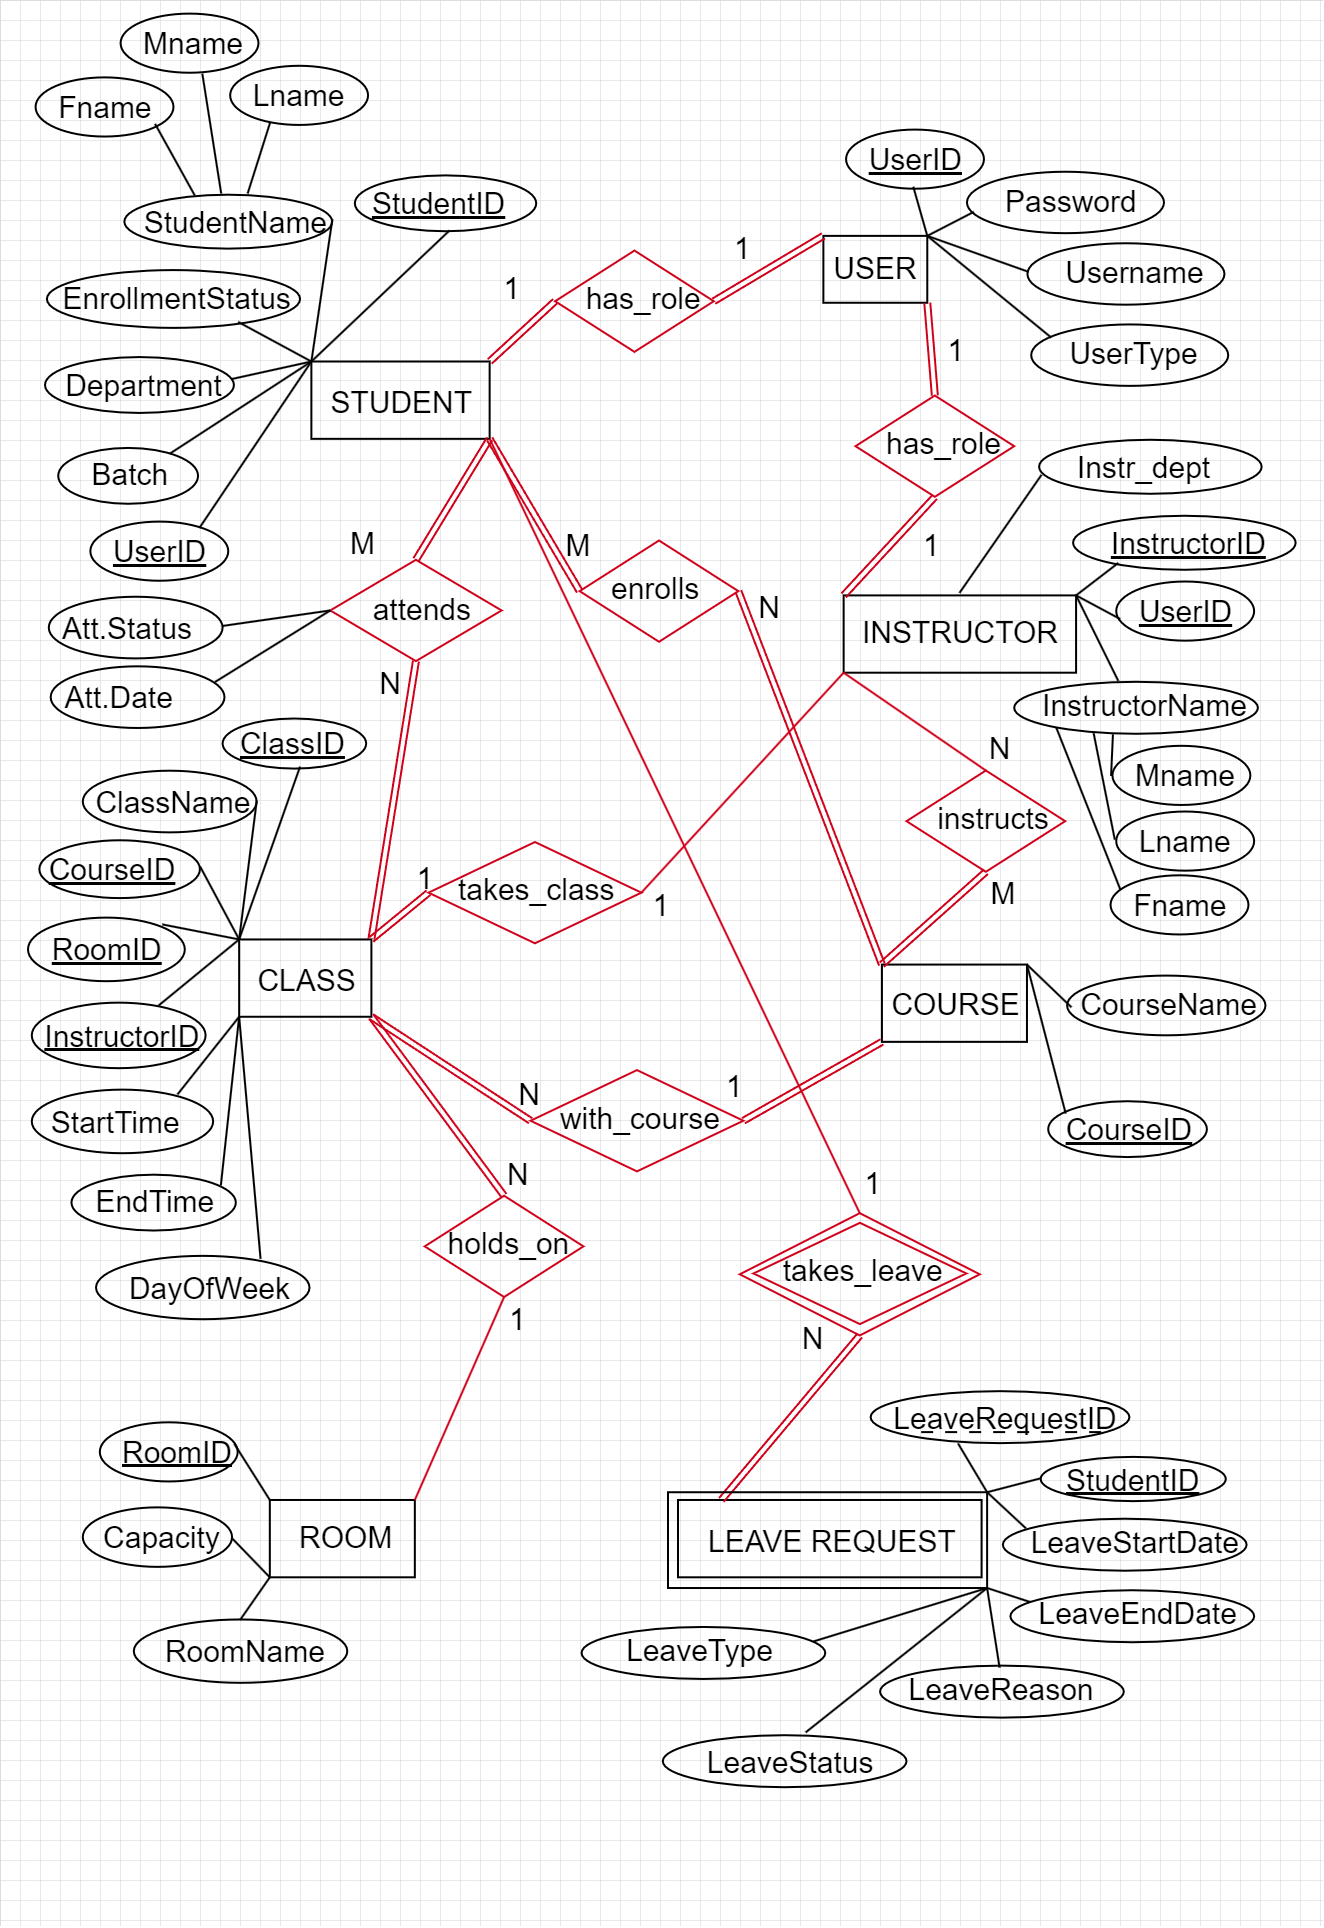
\includegraphics[width=1.1\textwidth, center]{er}
\end{figure}

\newpage
\section*{\huge{Relational Schema}}
\thispagestyle{empty}
\begin{figure}[H]
    \centering
    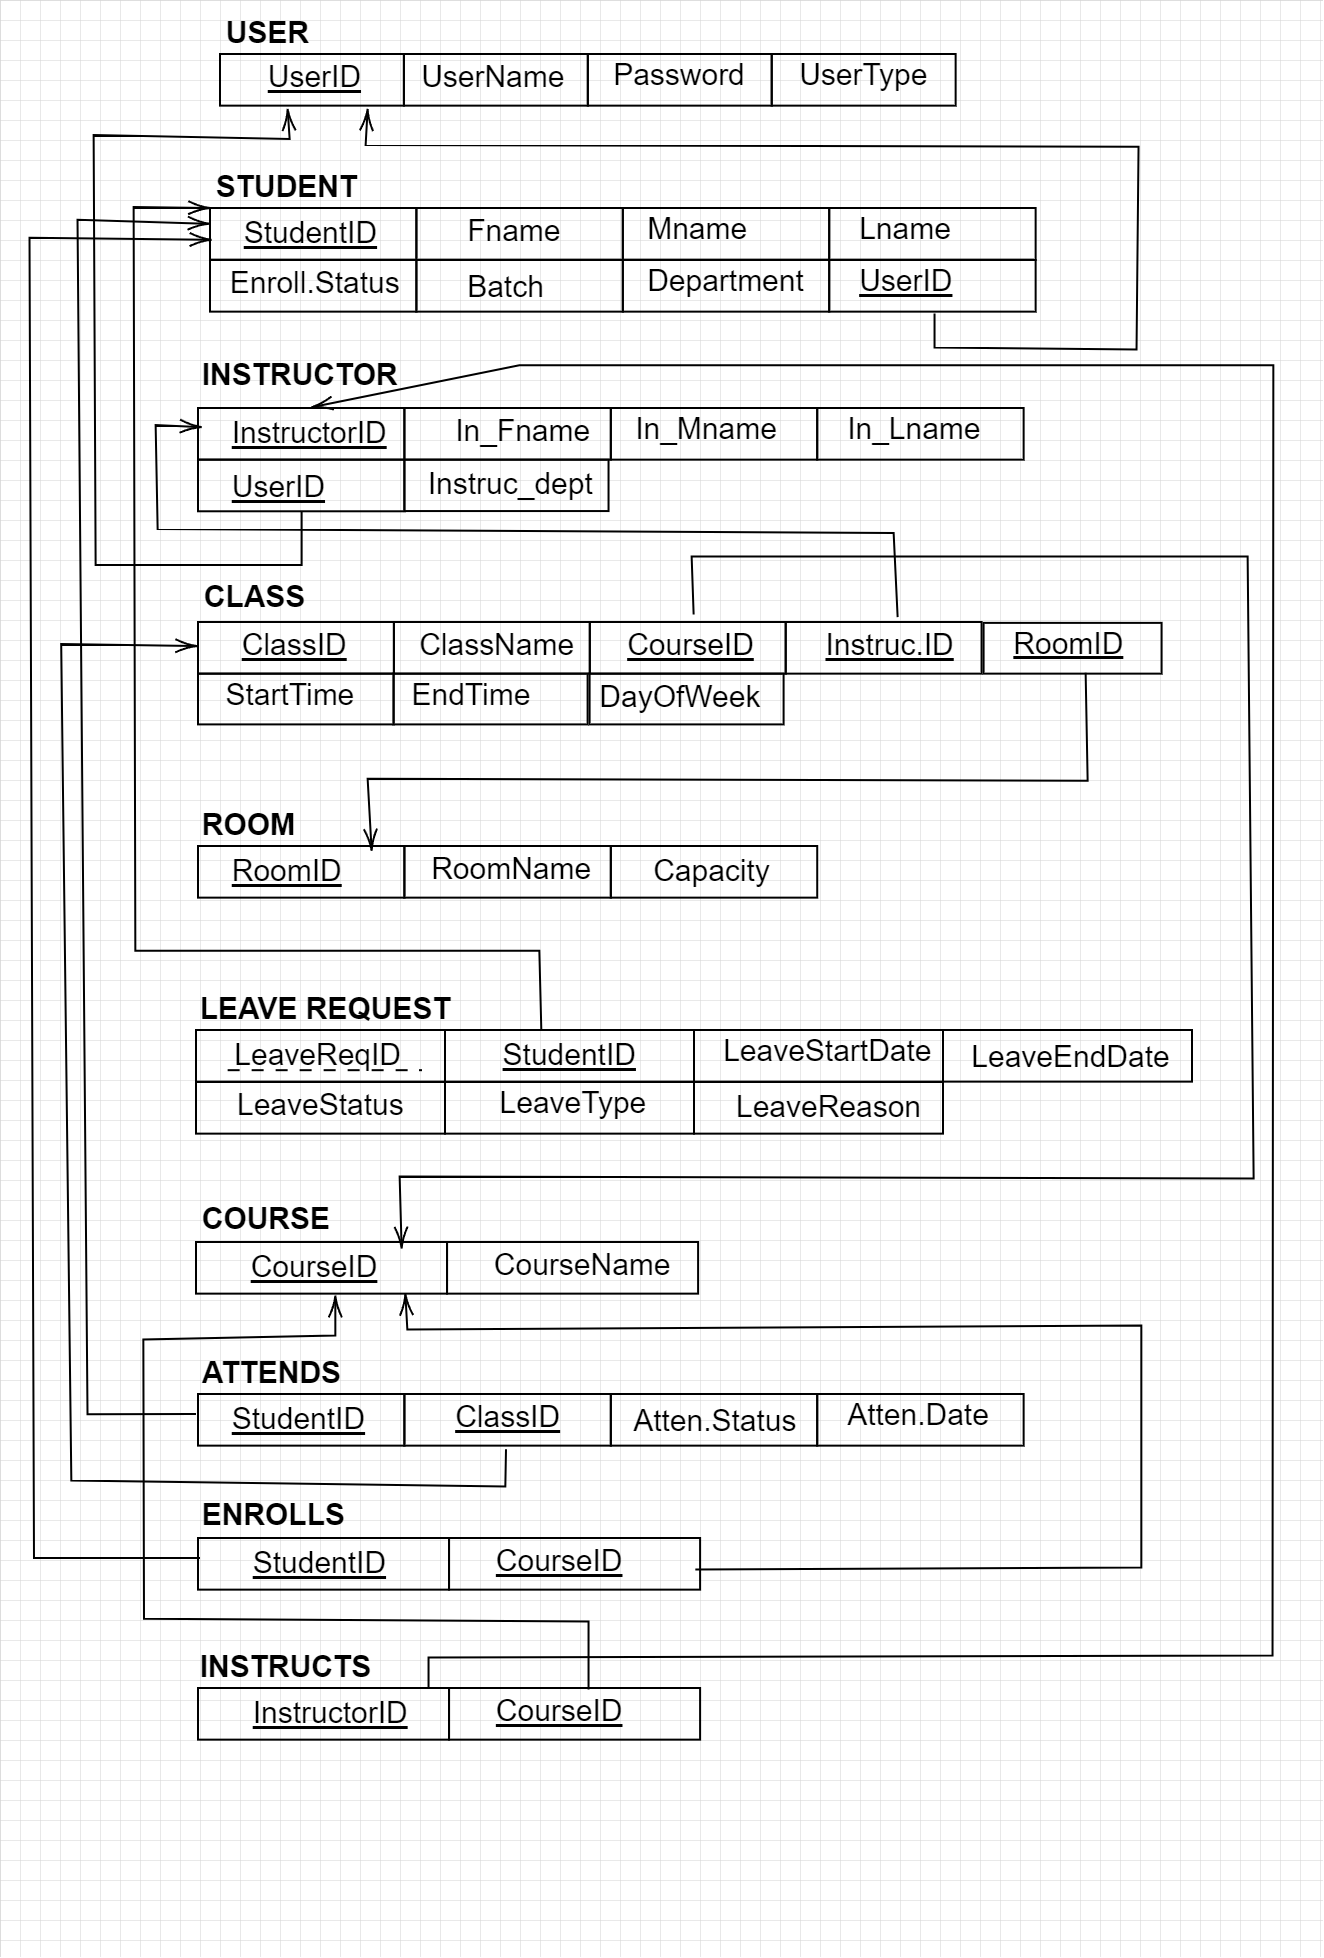
\includegraphics[width=1.1\textwidth, center]{rel}
\end{figure}



\newpage
\section*{\huge{Physical Data Model}}

\subsection*{\LARGE{Entities and Attributes:}}

\textbf{User:}

\begin{table}[H]
\centering
\begin{large}
\begin{tabular}{|l|l|l|}
\hline
\textbf{Attribute Name} & \textbf{Data Type} & \textbf{Key Type} \\ \hline
UserID & varchar& Primary Key \\\hline
Username & varchar & Non-key\\\hline
Password & varchar& Non-key\\\hline
UserType & varchar& Non-key\\ \hline
\end{tabular}
\end{large}
\end{table}



\textbf{Student:}
\begin{table}[H]
\centering
\begin{large}
\begin{tabular}{|l|l|l|}
\hline
\textbf{Attribute Name} & \textbf{Data Type} & \textbf{Key Type} \\ \hline
StudentID & varchar & Primary Key \\\hline
Fname & varchar & Non-key\\\hline
Mname & varchar & Non-key\\\hline
Lname & varchar & Non-Key \\\hline
Enroll.status & varchar & Non-key\\\hline
Batch & varchar & Non-key\\\hline
Department & varchar & Non-key\\ \hline
UserID & varchar & Foreign Key\\ \hline
\end{tabular}
\end{large}
\end{table}

\textbf{Instructor:}
\begin{table}[H]
\centering
\begin{large}
\begin{tabular}{|l|l|l|}
\hline
\textbf{Attribute Name} & \textbf{Data Type} & \textbf{Key Type} \\ \hline
InstructorID & varchar & Primary Key \\\hline
Instruc.Fname & varchar & Non-key\\\hline
Instruc.Mname & varchar & Non-key\\ \hline
Instruc.Lname & varchar & Non-Key \\ \hline
Instruc.Dept & varchar & Non-key\\  \hline
UserID & varchar & Foreign key\\ \hline
\end{tabular}
\end{large}
\end{table}



\textbf{Class:}
\begin{table}[H]
\centering
\begin{large}
\begin{tabular}{|l|l|l|}
\hline
\textbf{Attribute Name} & \textbf{Data Type} & \textbf{Key Type} \\ \hline
ClassID & varchar & Primary Key \\ \hline
ClassName & varchar & Non-key\\ \hline
CourseID & varchar & Foreign key\\ \hline
InstrucID & varchar & Foreign key \\ \hline
RoomID & varchar & Foreign key\\ \hline
StartTime & time & Non-key\\ \hline
EndTime & time & Non-key\\  \hline
DayOfWeek & varchar & Foreign Key\\ \hline
\end{tabular}
\end{large}
\end{table}


\textbf{Room:}
\begin{table}[H]
\centering
\begin{large}
\begin{tabular}{|l|l|l|}
\hline
\textbf{Attribute Name} & \textbf{Data Type} & \textbf{Key Type} \\ \hline
RoomID & varchar & Primary Key \\ \hline
RoomName & varchar & Non-key\\ \hline
Capacity & int & Non-key\\ \hline
\end{tabular}
\end{large}
\end{table}

\newpage
\textbf{Leave Request:}
\begin{table}[H]
\centering
\begin{large}
\begin{tabular}{|l|l|l|}
\hline
\textbf{Attribute Name} & \textbf{Data Type} & \textbf{Key Type} \\ \hline
LeaveReqID & varchar & Partial Key \\ \hline
StudentID & varchar & Foreign key\\ \hline
LeaveStartDate & date & Non-key \\ \hline
LeaveEndDate & date & Non-key\\ \hline
LeaveType & varchar & Non-key\\ \hline
LeaveReason & varchar & Non-key\\ \hline
LeaveStatus & varchar & Non-Key\\ \hline
\end{tabular}
\end{large}
\end{table}

\textbf{Course:}
\begin{table}[H]
\centering
\begin{large}
\begin{tabular}{|l|l|l|}
\hline
\textbf{Attribute Name} & \textbf{Data Type} & \textbf{Key Type} \\ \hline
CourseID & varchar & Primary Key \\ \hline
CourseName & varchar & Non-Key\\ \hline
\end{tabular}
\end{large}
\end{table}


\textbf{Attends:}
\begin{table}[H]
\centering
\begin{large}
\begin{tabular}{|l|l|l|}
\hline
\textbf{Attribute Name} & \textbf{Data Type} & \textbf{Key Type} \\ \hline
StudentID & varchar & Foreign Key \\ \hline
ClassID & varchar & Foreign key\\ \hline
Atten.Status & varchar & Non-key\\ \hline
Atten.Date & date & Non-Key\\ \hline
\end{tabular}
\end{large}
\end{table}



\textbf{Enrolls:}
\begin{table}[H]
\centering
\begin{large}
\begin{tabular}{|l|l|l|}
\hline
\textbf{Attribute Name} & \textbf{Data Type} & \textbf{Key Type} \\ \hline
StudentID & varchar & Foreign Key \\ \hline
CourseID & varchar & Foreign Key\\ \hline
\end{tabular}
\end{large}
\end{table}


\textbf{Instructs:}
\begin{table}[H]
\centering
\begin{large}
\begin{tabular}{|l|l|l|}
\hline
\textbf{Attribute Name} & \textbf{Data Type} & \textbf{Key Type} \\ \hline
InstructorID & varchar & Foreign Key \\ \hline
CourseID & varchar & Foreign Key\\ \hline
\end{tabular}
\end{large}
\end{table}

\newpage

\section*{\LARGE{Relationships:}}

\subsection*{User-Student (1:1):}
\begin{large}
Relation specifying UserType of a user(here Student). Each student in the system corresponds to exactly one user for authentication and access purpose.
Similarly each user account is associated with exactly one student. 
\end{large}

\subsection*{User-Instructor (1:1):}
\begin{large}
Relation specifying UserType of a user(here Instructor). Each instructor in the system corresponds to exactly one user similarly to that of student-user relationship.
Similarly each user account is associated with exactly one instructor. 
\end{large}

\subsection*{Student-Course (M:N):}
\begin{large}
Describes the registered courses of a student. A student can be enrolled in multiple courses and a course can have multiple students 
enrolled in it. 
\end{large}

\subsection*{Course-Instructor (M:N):}
\begin{large}
Describes the courses which are taught by an Instructor. An instructor can teach multiple courses and a course can be taught by multiple instructors.
\end{large}

\subsection*{Student-Class (M:N):}
\begin{large}
Relation describring the classes attended by a student. A student can attend multiple classes and a class can be attended by multiple students.
\end{large}

\subsection*{Instructor-Class (1:N):}
\begin{large}
Relation describring the classes handled by an Instructor. Each class is typically taught by one instructor and each instructor teaches multiple classes.
\end{large}

\subsection*{Class-Course (N:1):}
\begin{large}
Describes the courses taught in a class. Each class is exactly associated with one course, but a course may have multiple classes associated 
with it.
\end{large}

\subsection*{Class-Room (N:1):}
\begin{large}
Describes the rooms in which classes are taught. Similarly, each class is typically conducted in one room, but a room may host multiple classes.
\end{large}

\subsection*{Student-Leave Request (1:N):}
\begin{large}
Relation providing all the leave requests of a student. A student can submit multiple leave requests, but each leave request is associated with exactly 
one student. 
\end{large}


\newpage
\section*{\huge{Population Queries(MySQL):}}

\begin{itemize}
    \item \thispagestyle{empty}
    {\large{Database and tables}}
    \begin{figure}[H]
        \centering
        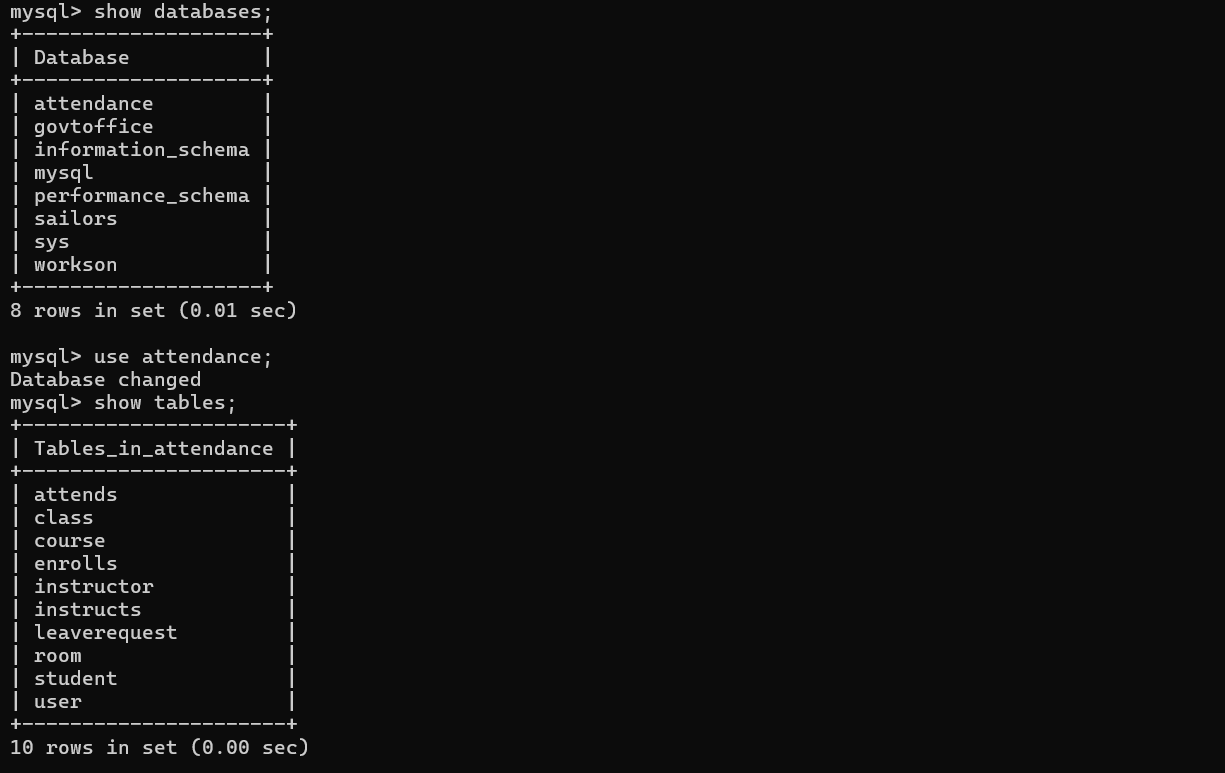
\includegraphics[width=1.1\textwidth, center]{1}
    \end{figure}

    \item \thispagestyle{empty}
    {\large{Example entries in course table}}
    \begin{figure}[H]
        \centering
        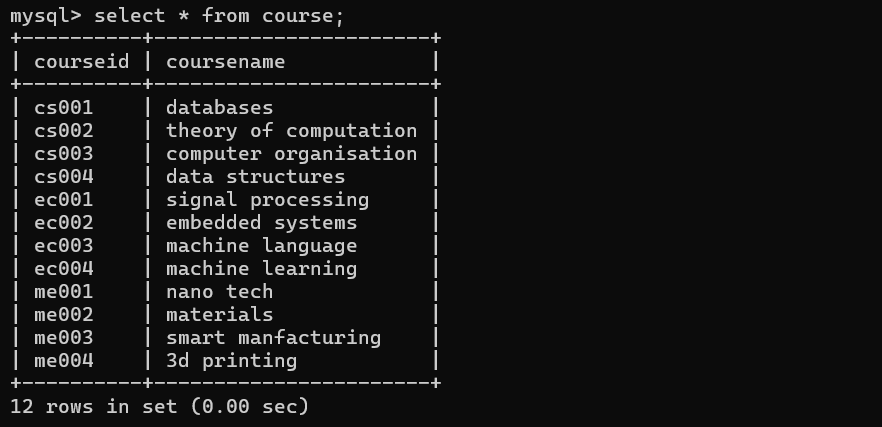
\includegraphics[width=1.1\textwidth, center]{2}
    \end{figure}

    \newpage

    \item \thispagestyle{empty}
    {\large{Example entries in student table}}
    \begin{figure}[H]
        \centering
        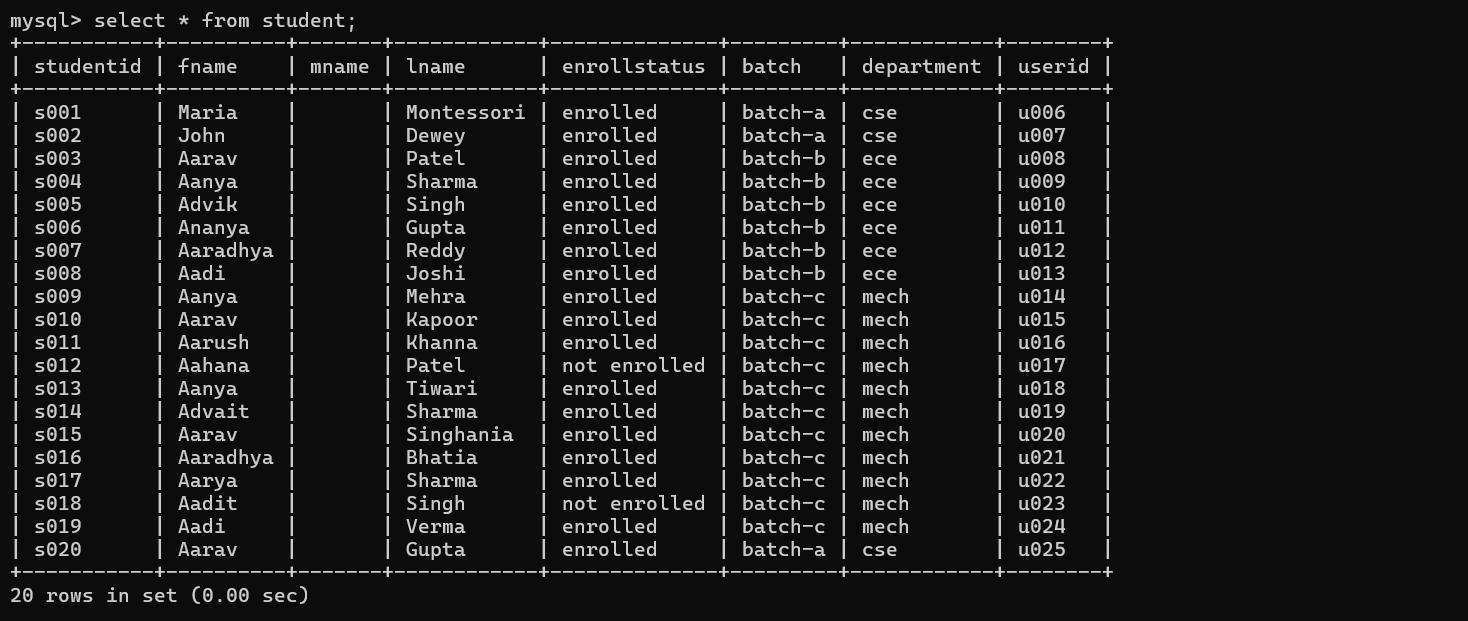
\includegraphics[width=1.1\textwidth, center]{3}
    \end{figure}

    \item \thispagestyle{empty}
    {\large{Example entries in user table}}
    \begin{figure}[H]
        \centering
        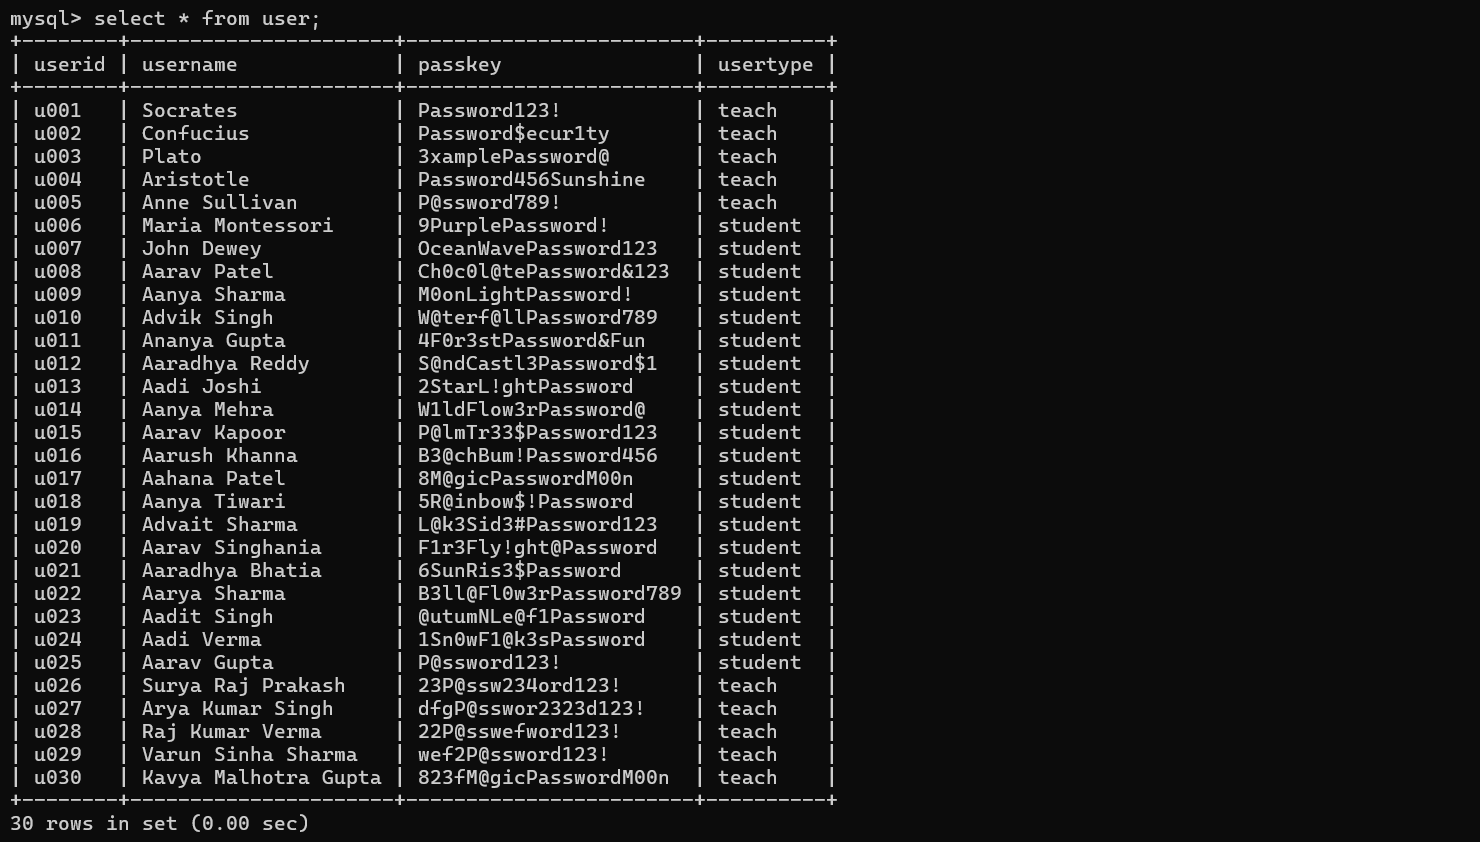
\includegraphics[width=1.1\textwidth, center]{4}
    \end{figure}

    \item \thispagestyle{empty}
    {\large{Example entries in instructor table}}
    \begin{figure}[H]
        \centering
        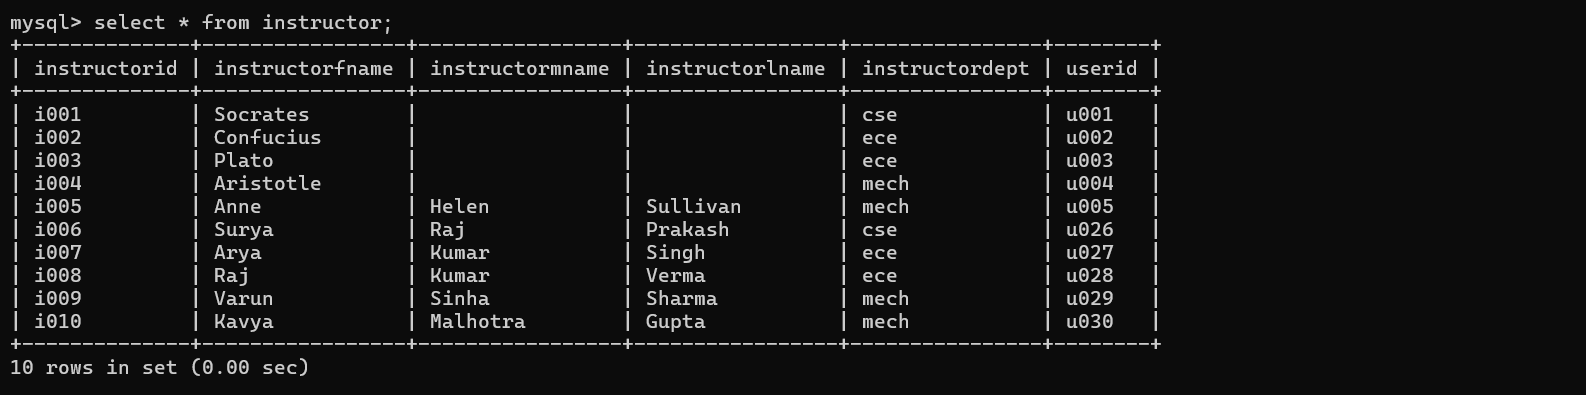
\includegraphics[width=1.1\textwidth, center]{5}
    \end{figure}

    \newpage

    \item \thispagestyle{empty}
    {\large{Example entries in attends table}}
    \begin{figure}[H]
        \centering
        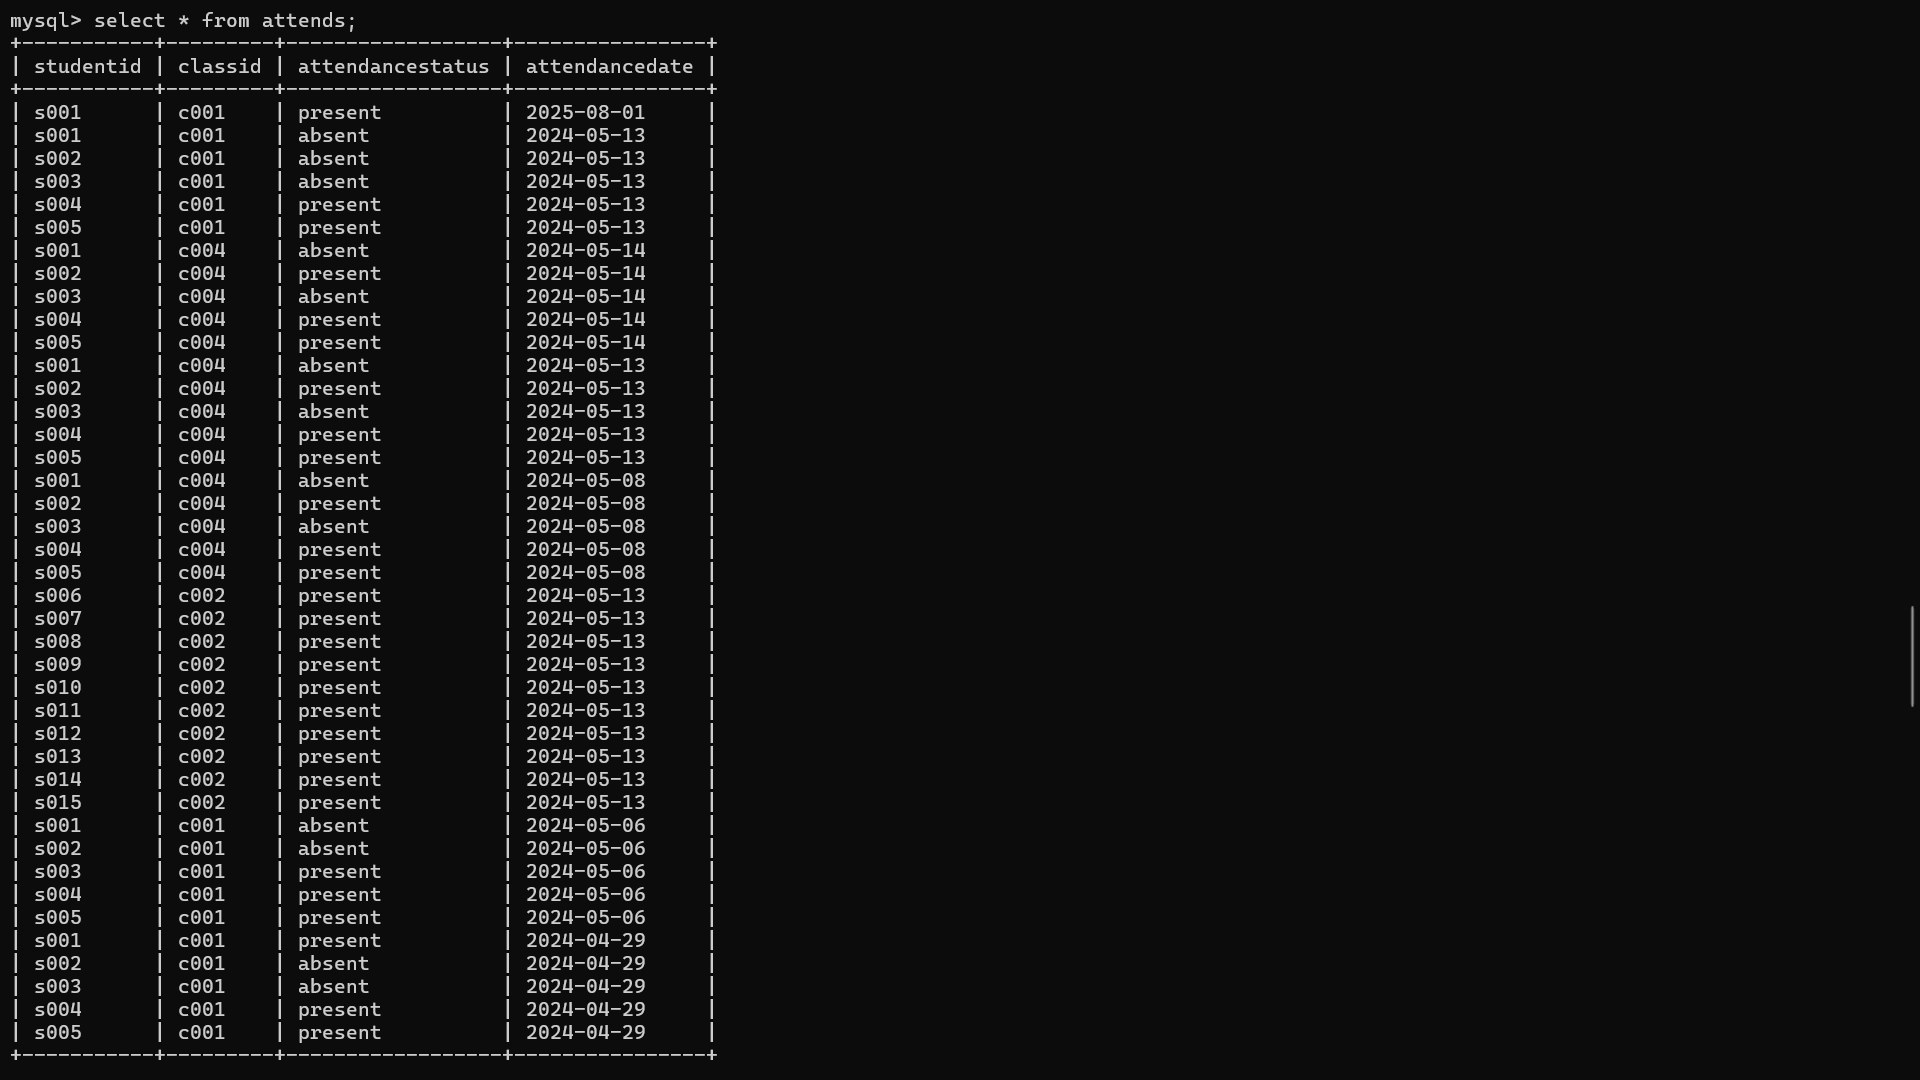
\includegraphics[width=1.1\textwidth, center]{6}
    \end{figure}

    \item \thispagestyle{empty}
    {\large{Example entries in leaverequest table}}
    \begin{figure}[H]
        \centering
        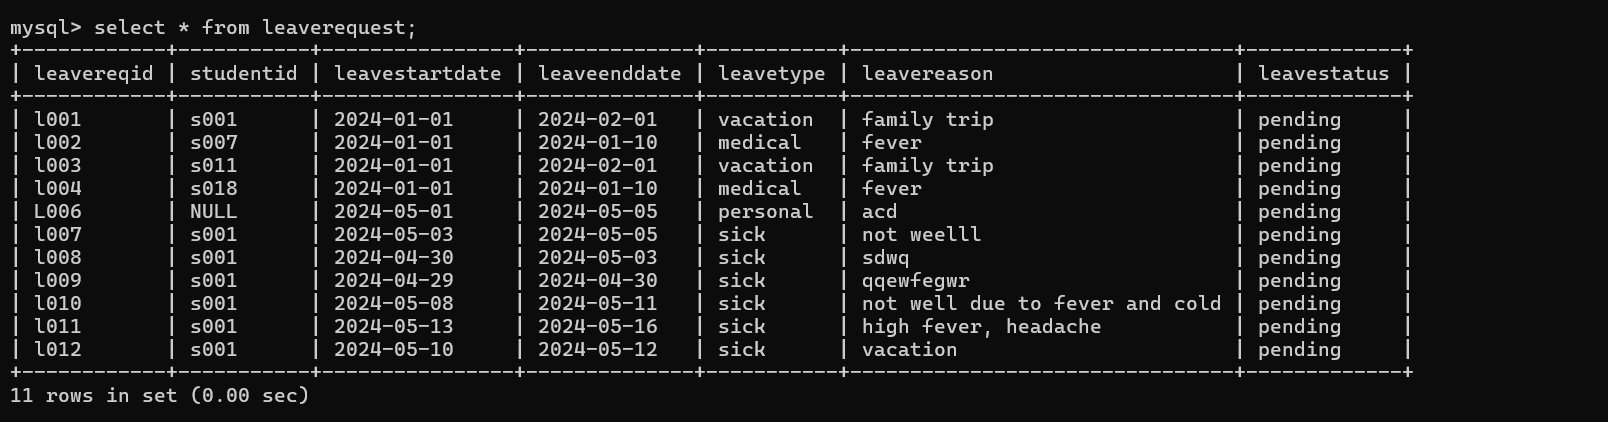
\includegraphics[width=1.1\textwidth, center]{7}
    \end{figure}

    \item \thispagestyle{empty}
    {\large{Example entries in instructs table}}
    \begin{figure}[H]
        \centering
        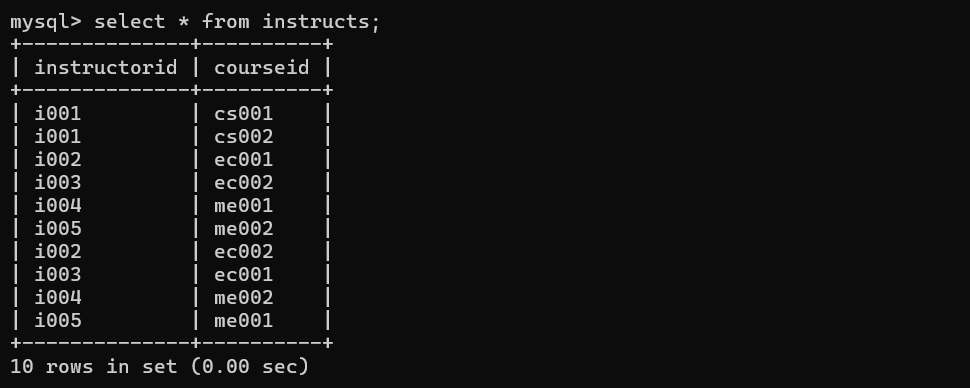
\includegraphics[width=1.1\textwidth, center]{8}
    \end{figure}
    
    \newpage

    \item \thispagestyle{empty}
    {\large{Example entries in room table}}
    \begin{figure}[H]
        \centering
        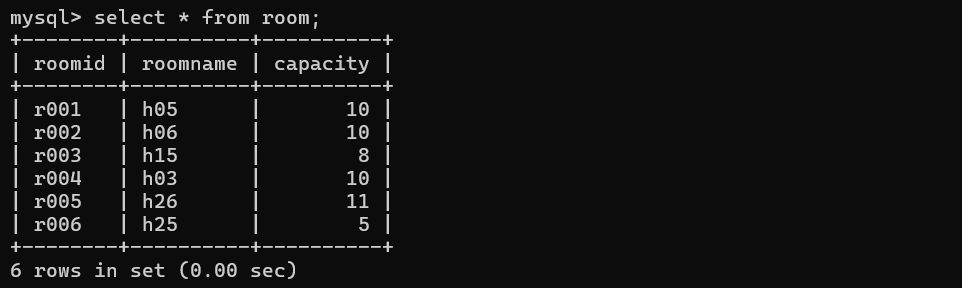
\includegraphics[width=1.1\textwidth, center]{9}
    \end{figure}

    \item \thispagestyle{empty}
    {\large{Example entries in enrolls table}}
    \begin{figure}[H]
        \centering
        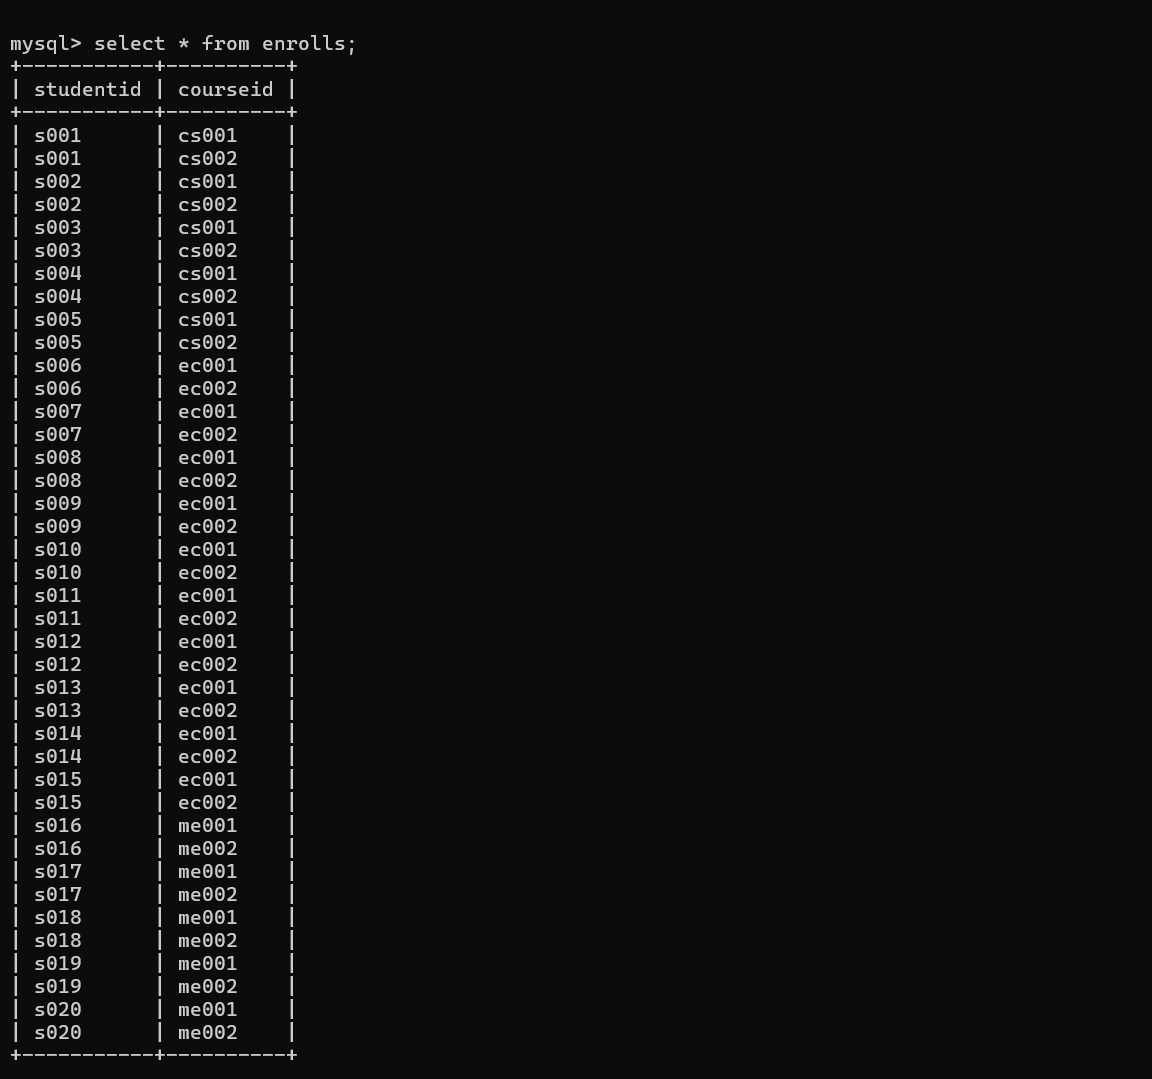
\includegraphics[width=1.1\textwidth, center]{10}
    \end{figure}
\end{itemize}

\newpage

\section*{\huge{Front-End:}}

\begin{itemize}
    \item \thispagestyle{empty}
    {\large{Running the application using "nodemon". It automatically restarts the node 
    application when a file change occurs}}
    \begin{figure}[H]
        \centering
        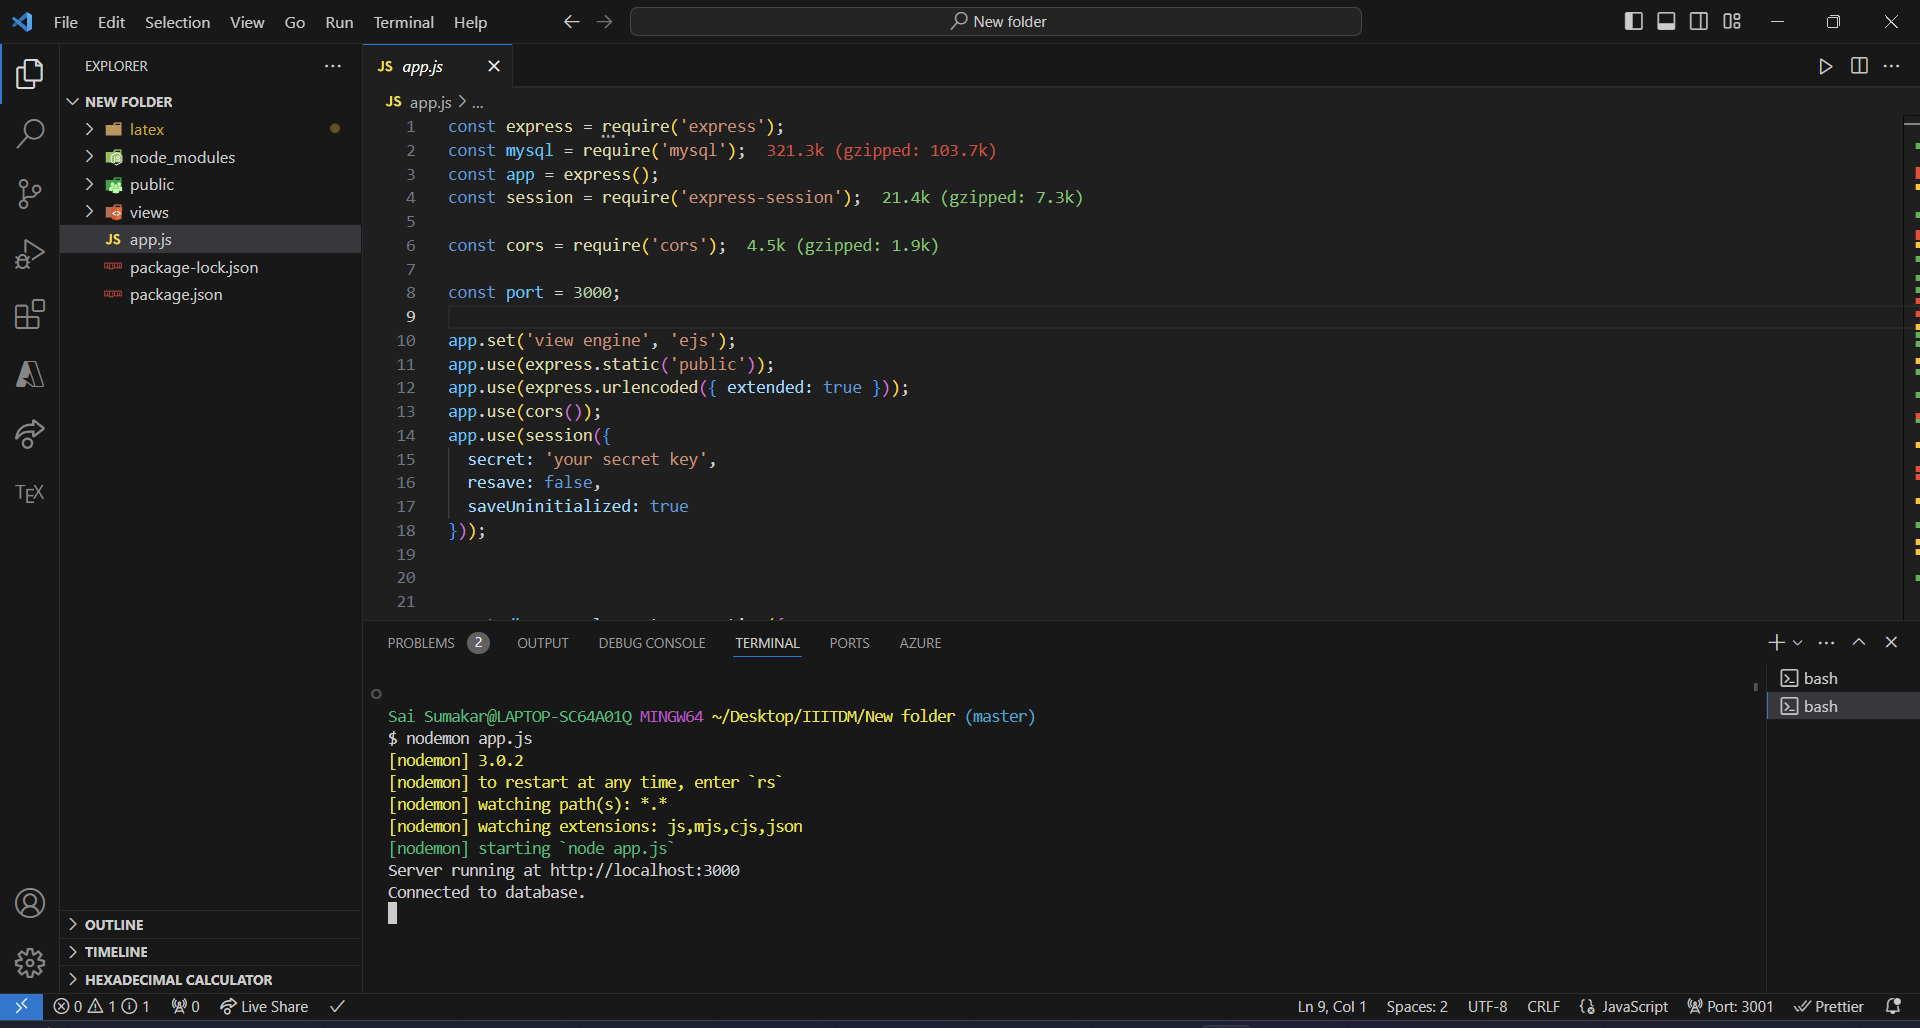
\includegraphics[width=1.1\textwidth, center]{11}
    \end{figure}

    \vspace*{2cm}

    \item \thispagestyle{empty}
    {\large{Landing Page(Login). Either a student or a faculty can login 
    using their credentials}}
    \begin{figure}[H]
        \centering
        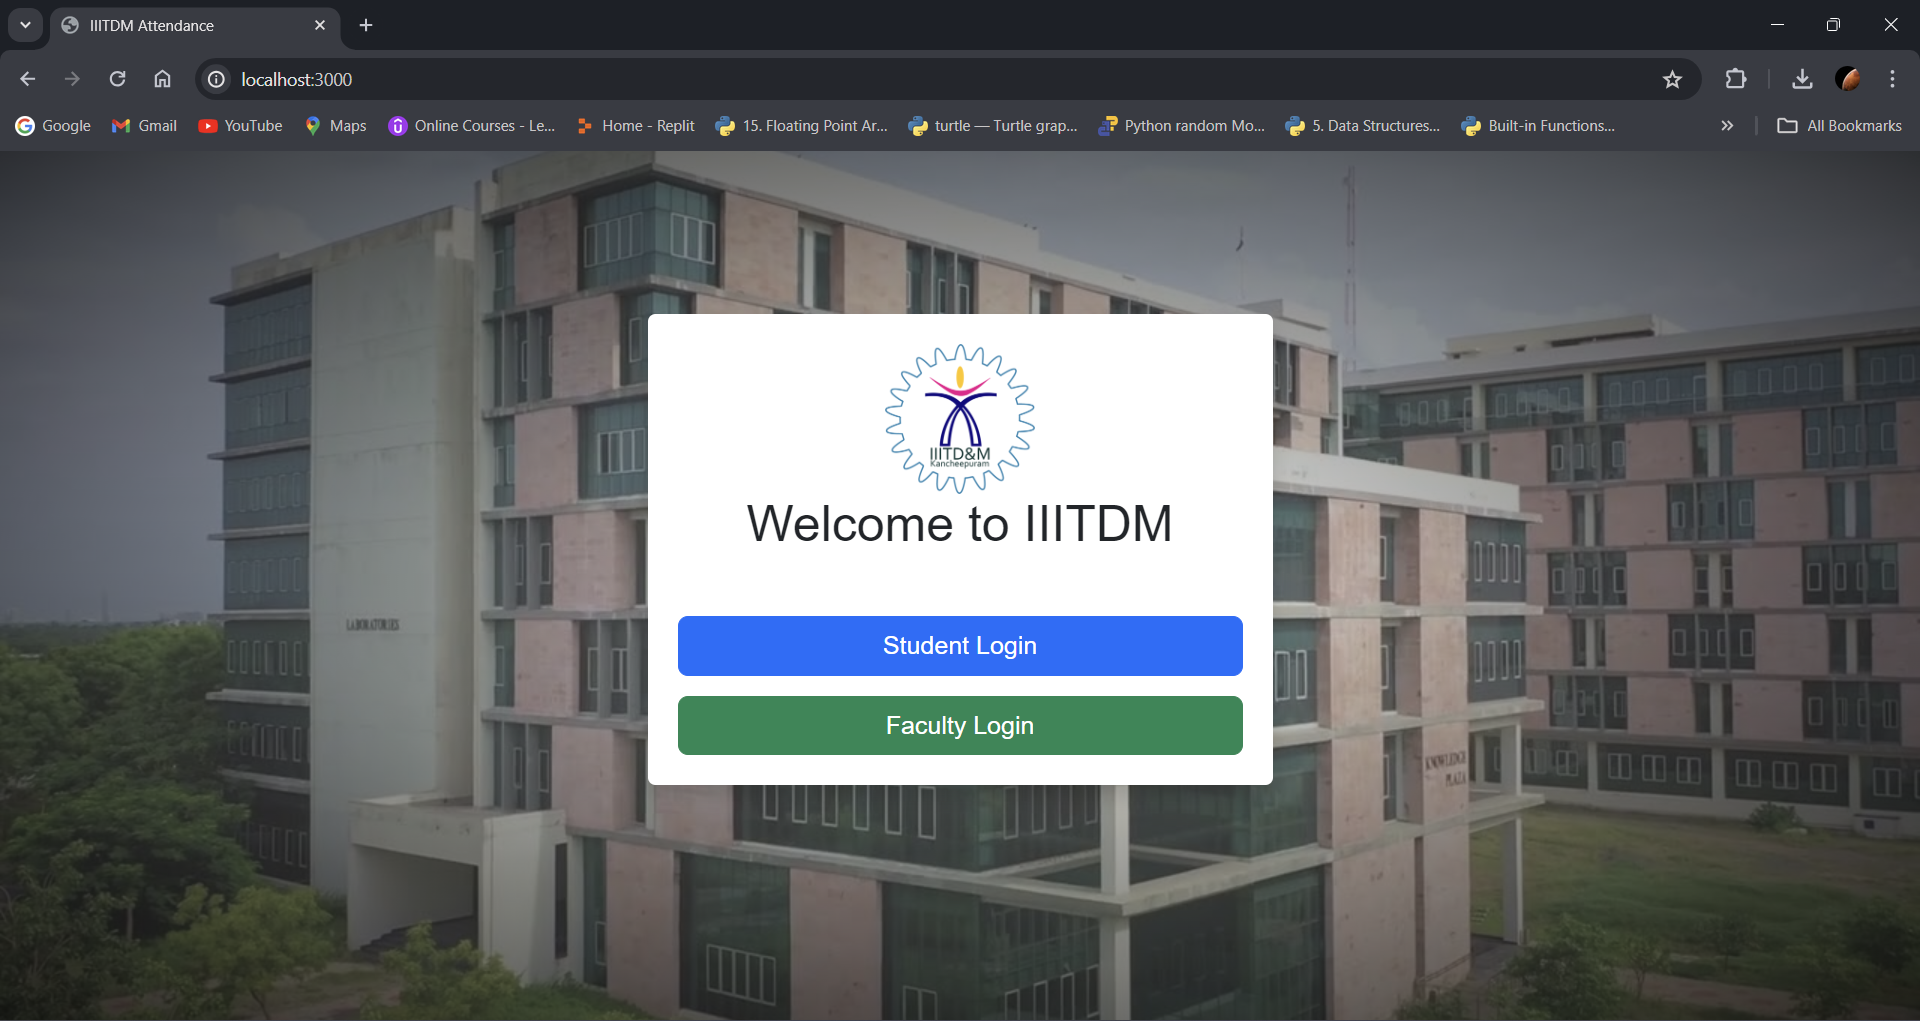
\includegraphics[width=1.1\textwidth, center]{12}
    \end{figure}

    \newpage

    \item \thispagestyle{empty}
    {\large{Student login Page}}
    \begin{figure}[H]
        \centering
        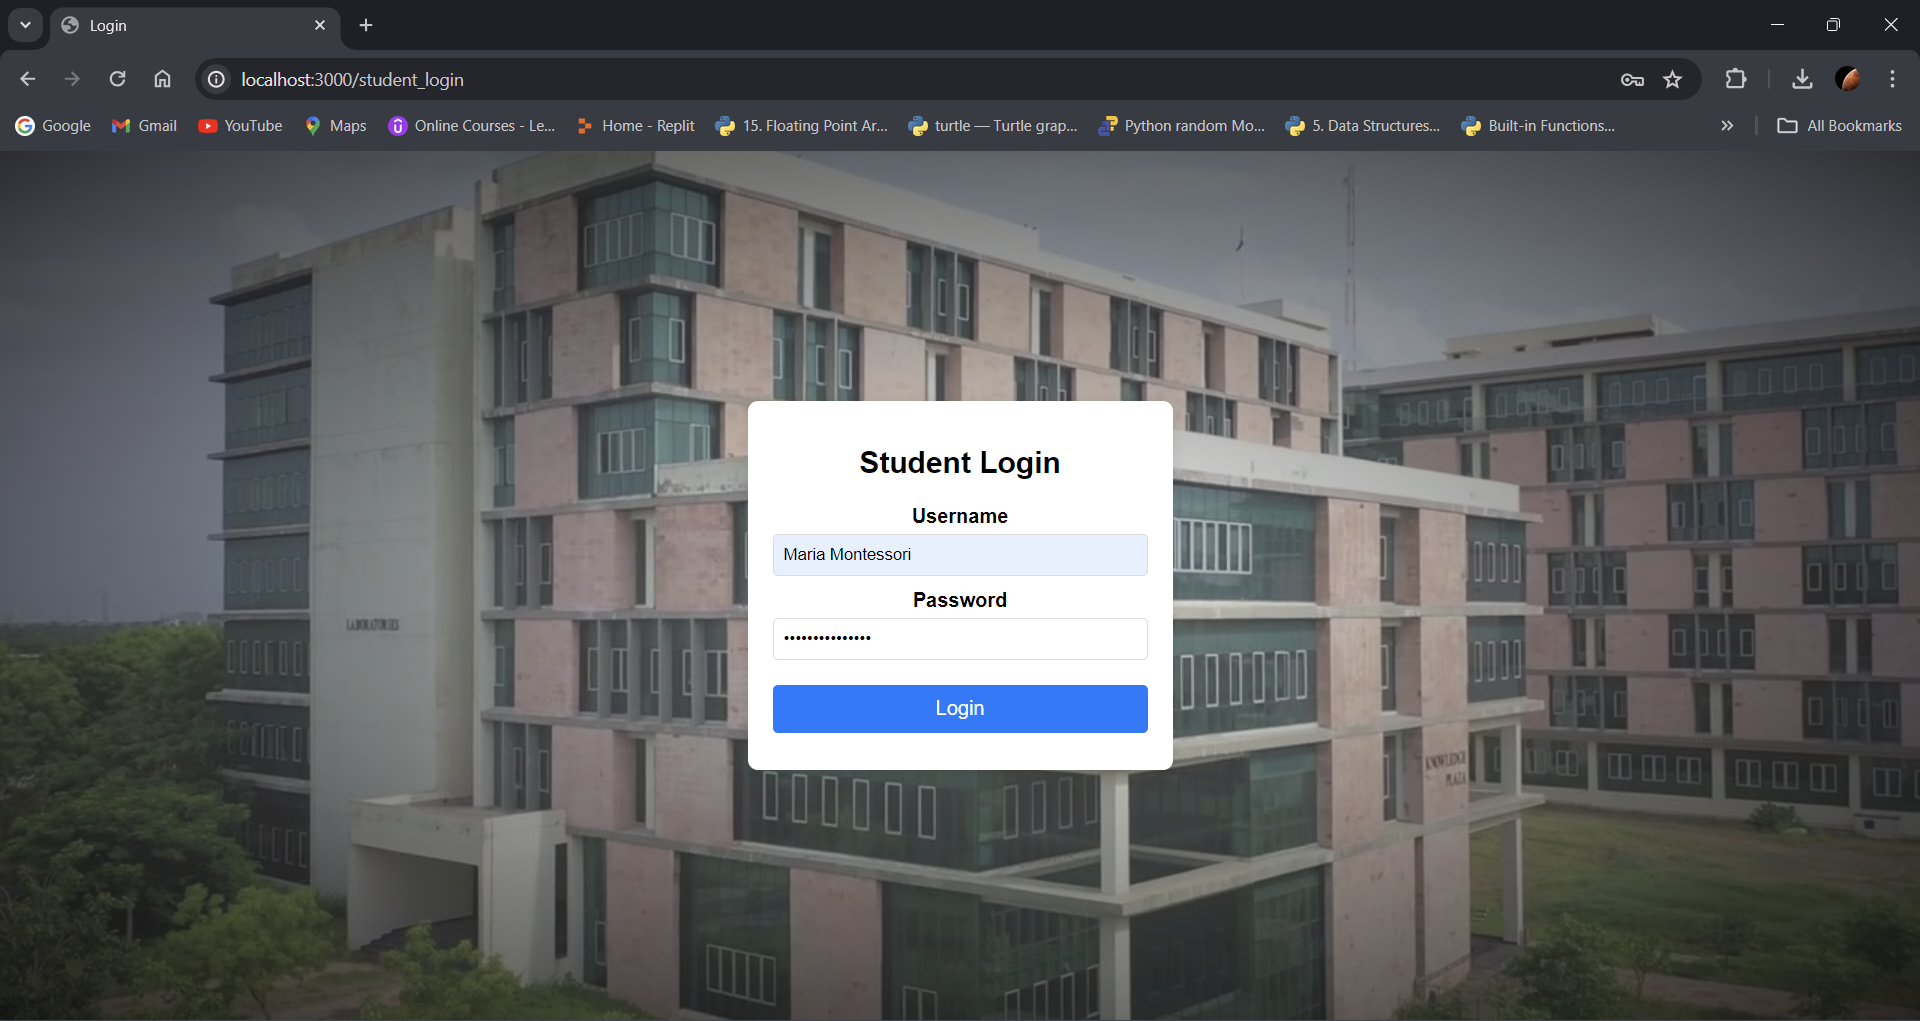
\includegraphics[width=1.1\textwidth, center]{13}
    \end{figure}

    \vspace*{2cm}

    \item \thispagestyle{empty}
    {\large{Student attendance Page showing the attendance of the student
    in their enrolled courses.}}
    \begin{figure}[H]
        \centering
        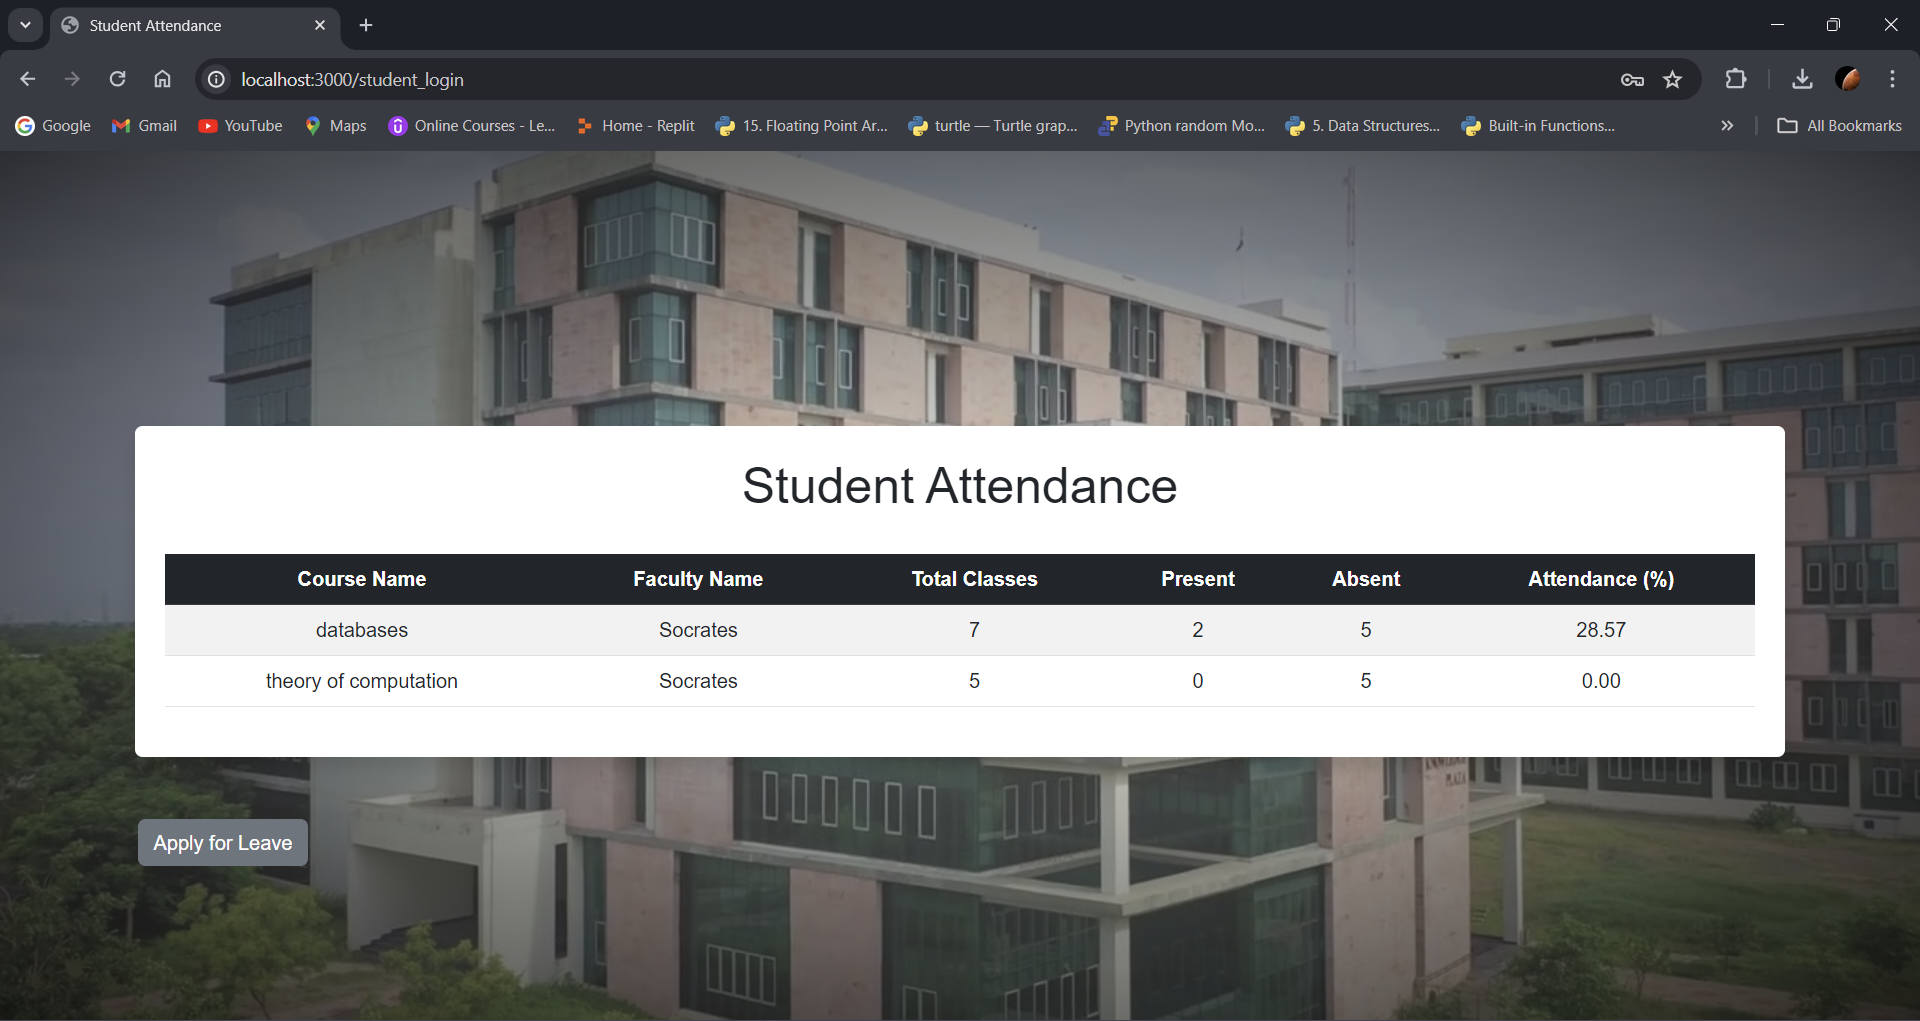
\includegraphics[width=1.1\textwidth, center]{14}
    \end{figure}

    \newpage

    \item \thispagestyle{empty}
    {\large{Leave Application Page}}
    \begin{figure}[H]
        \centering
        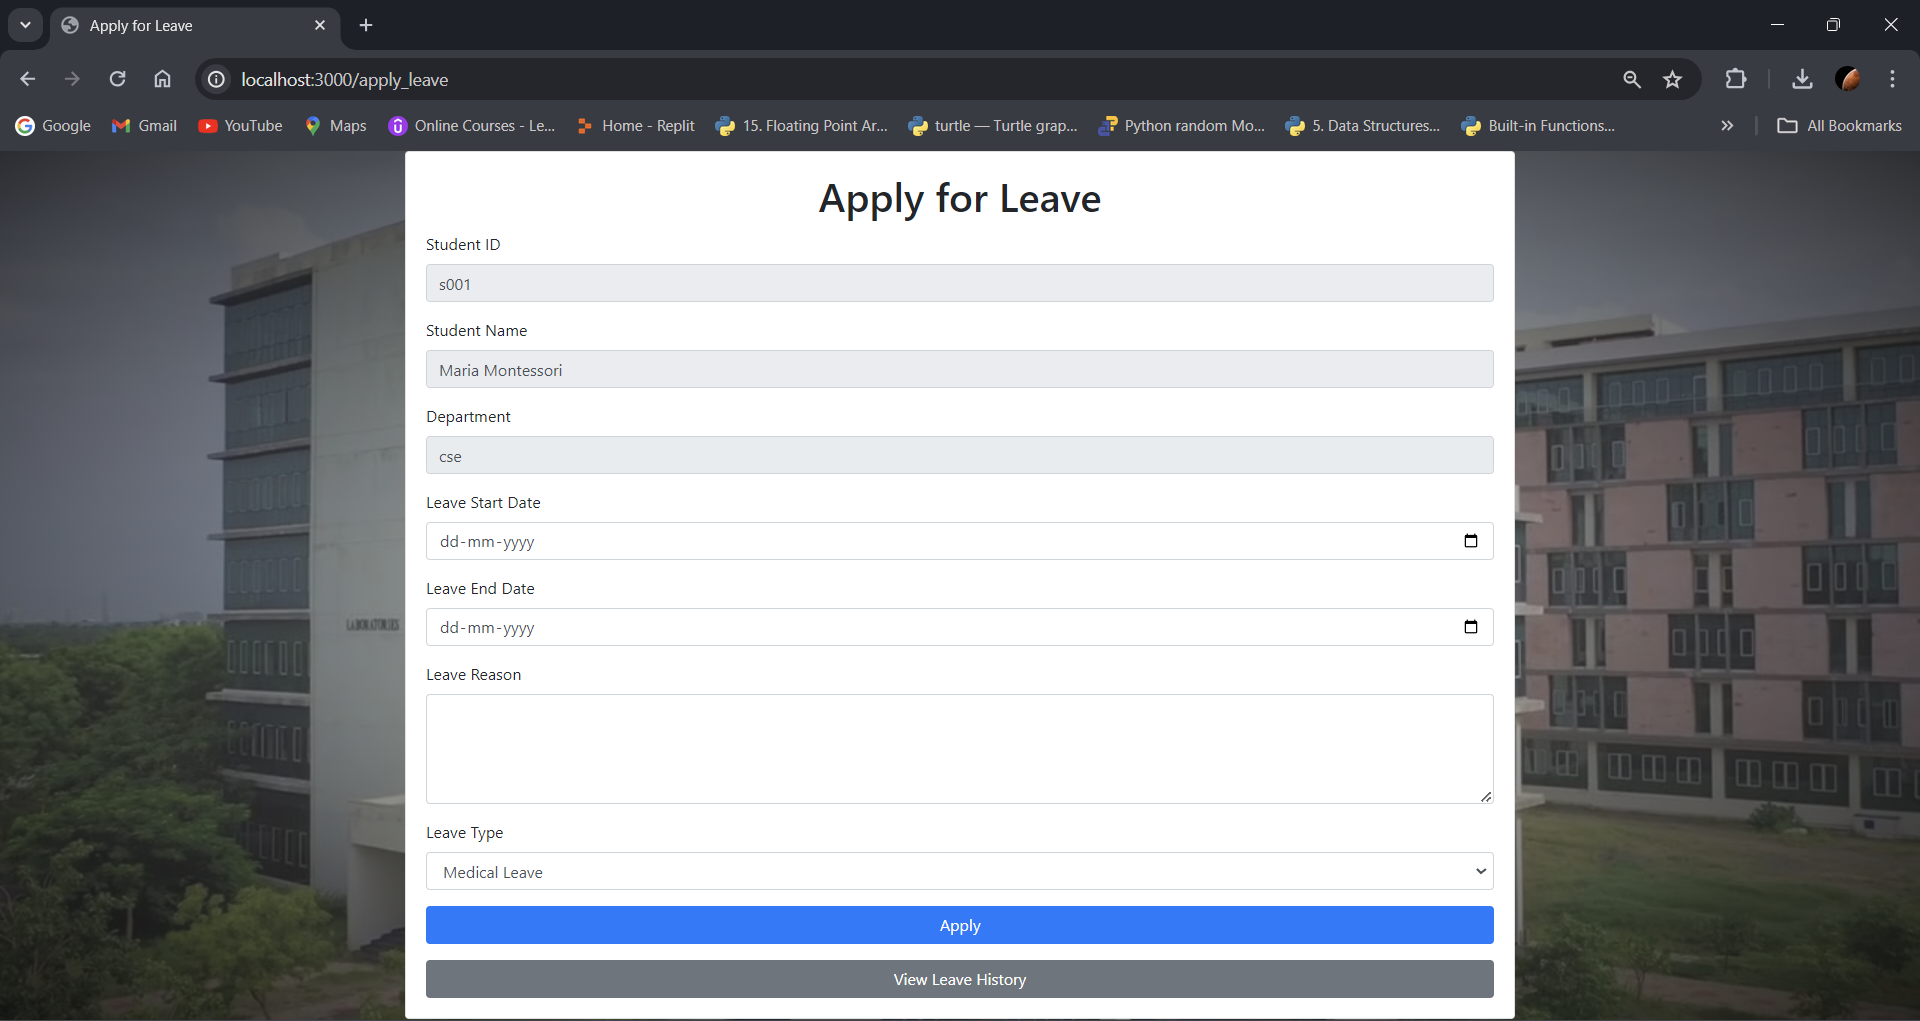
\includegraphics[width=1.1\textwidth, center]{15}
    \end{figure}
    
    \vspace*{2cm}

    \item \thispagestyle{empty}
    {\large{Leave History Page}}
    \begin{figure}[H]
        \centering
        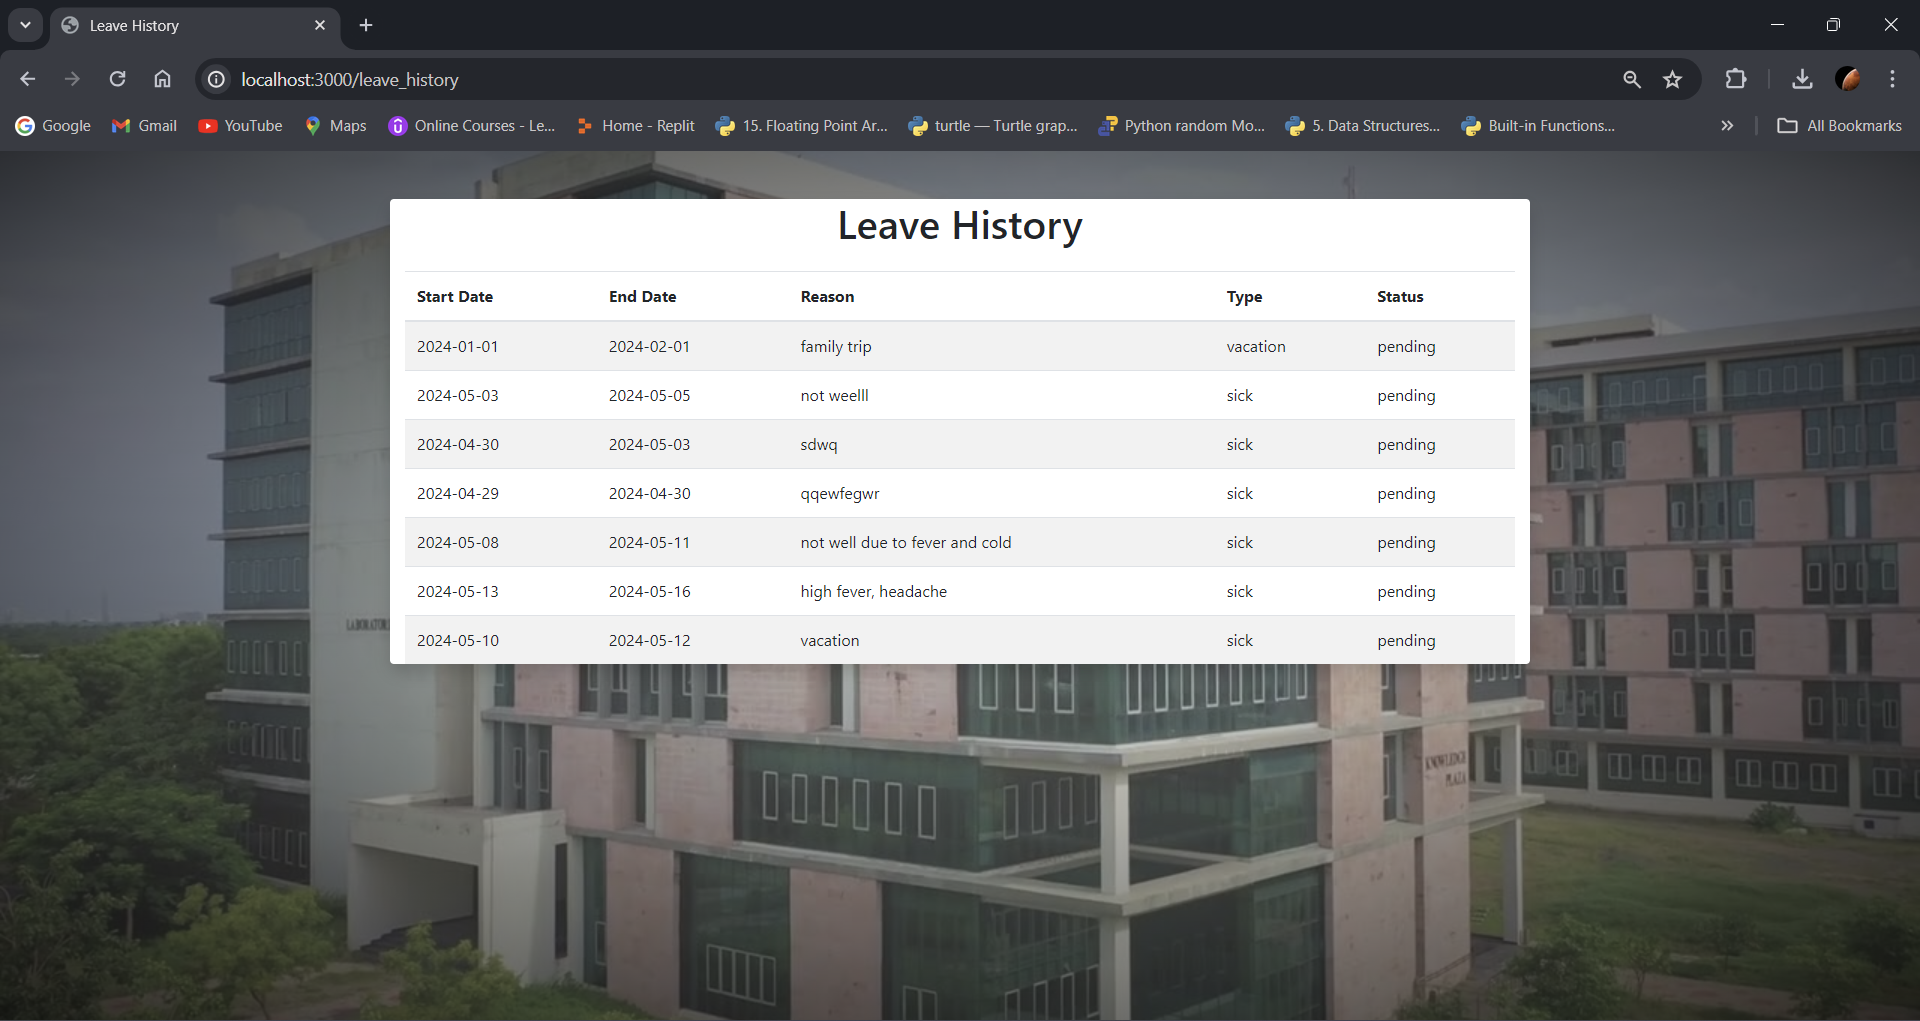
\includegraphics[width=1.1\textwidth, center]{16}
    \end{figure}
    
    \newpage

    \item \thispagestyle{empty}
    {\large{Faculty Login Page}}
    \begin{figure}[H]
        \centering
        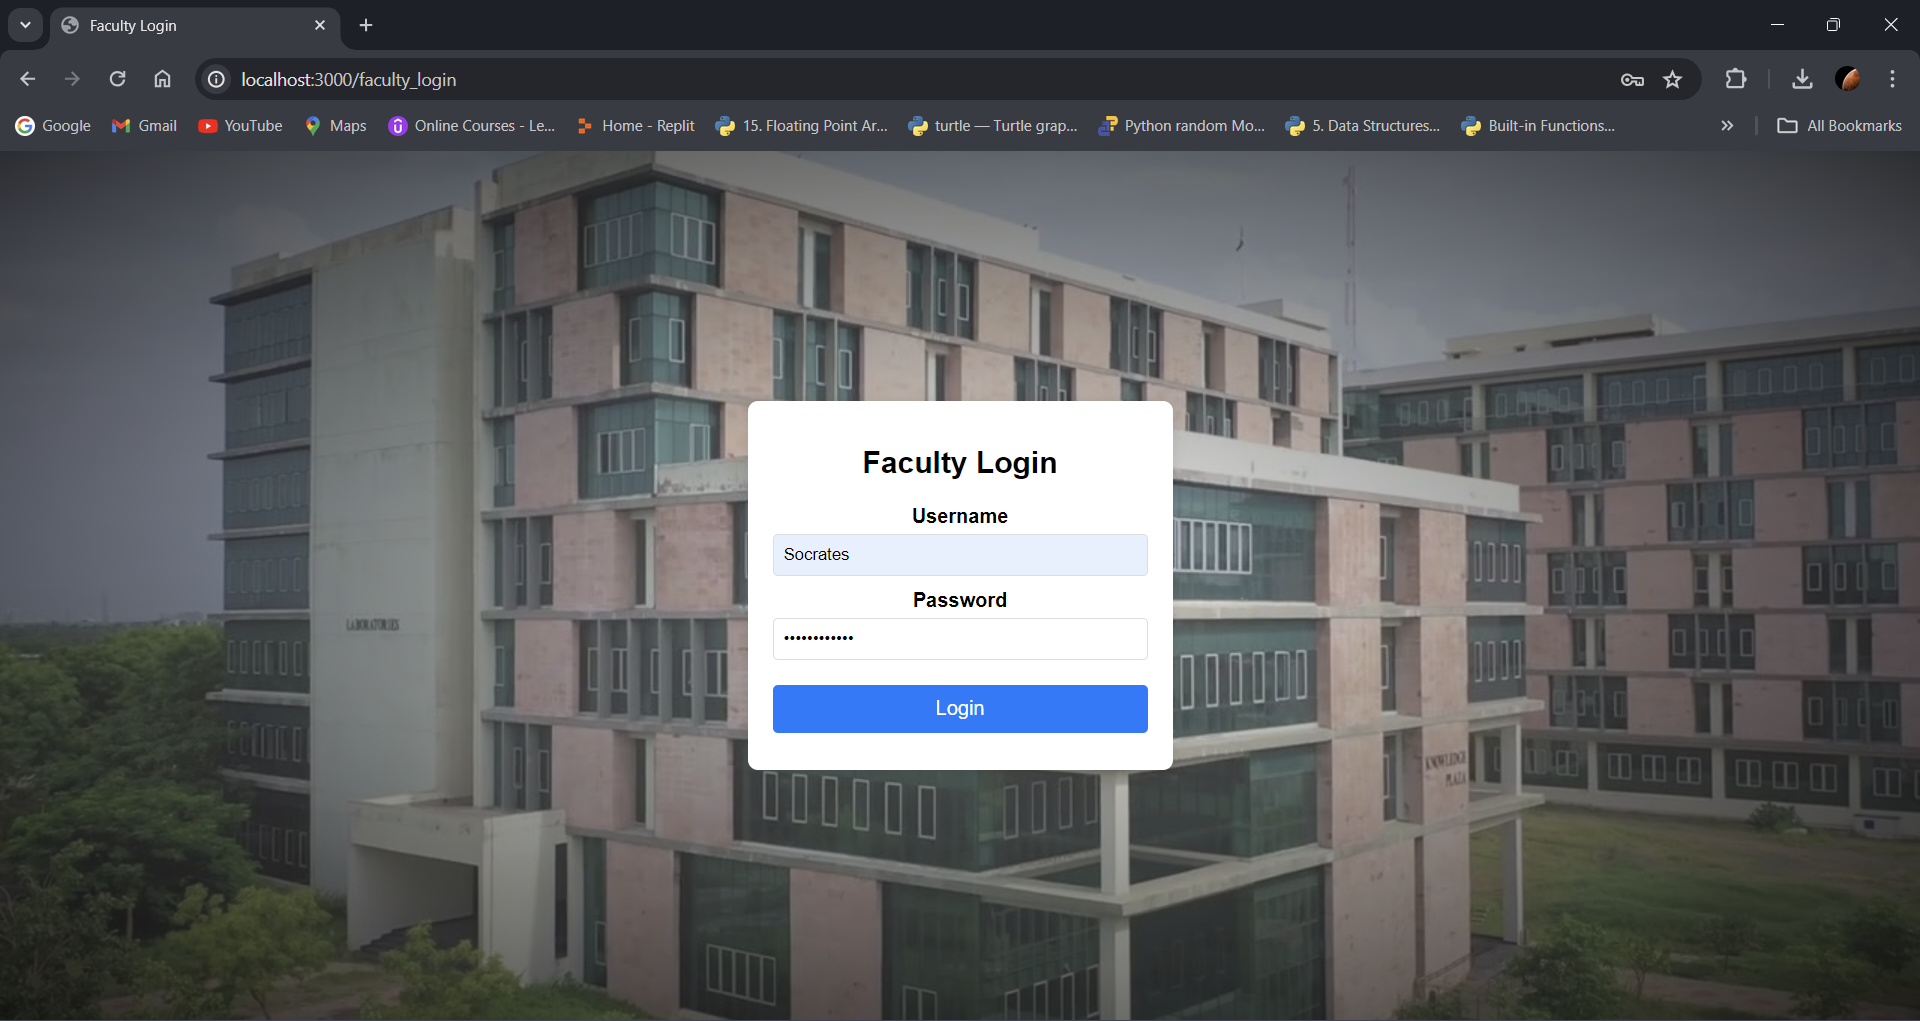
\includegraphics[width=1.1\textwidth, center]{17}
    \end{figure}

    \vspace*{2cm}

    \item \thispagestyle{empty}
    {\large{Attendance Marking Page}}
    \begin{figure}[H]
        \centering
        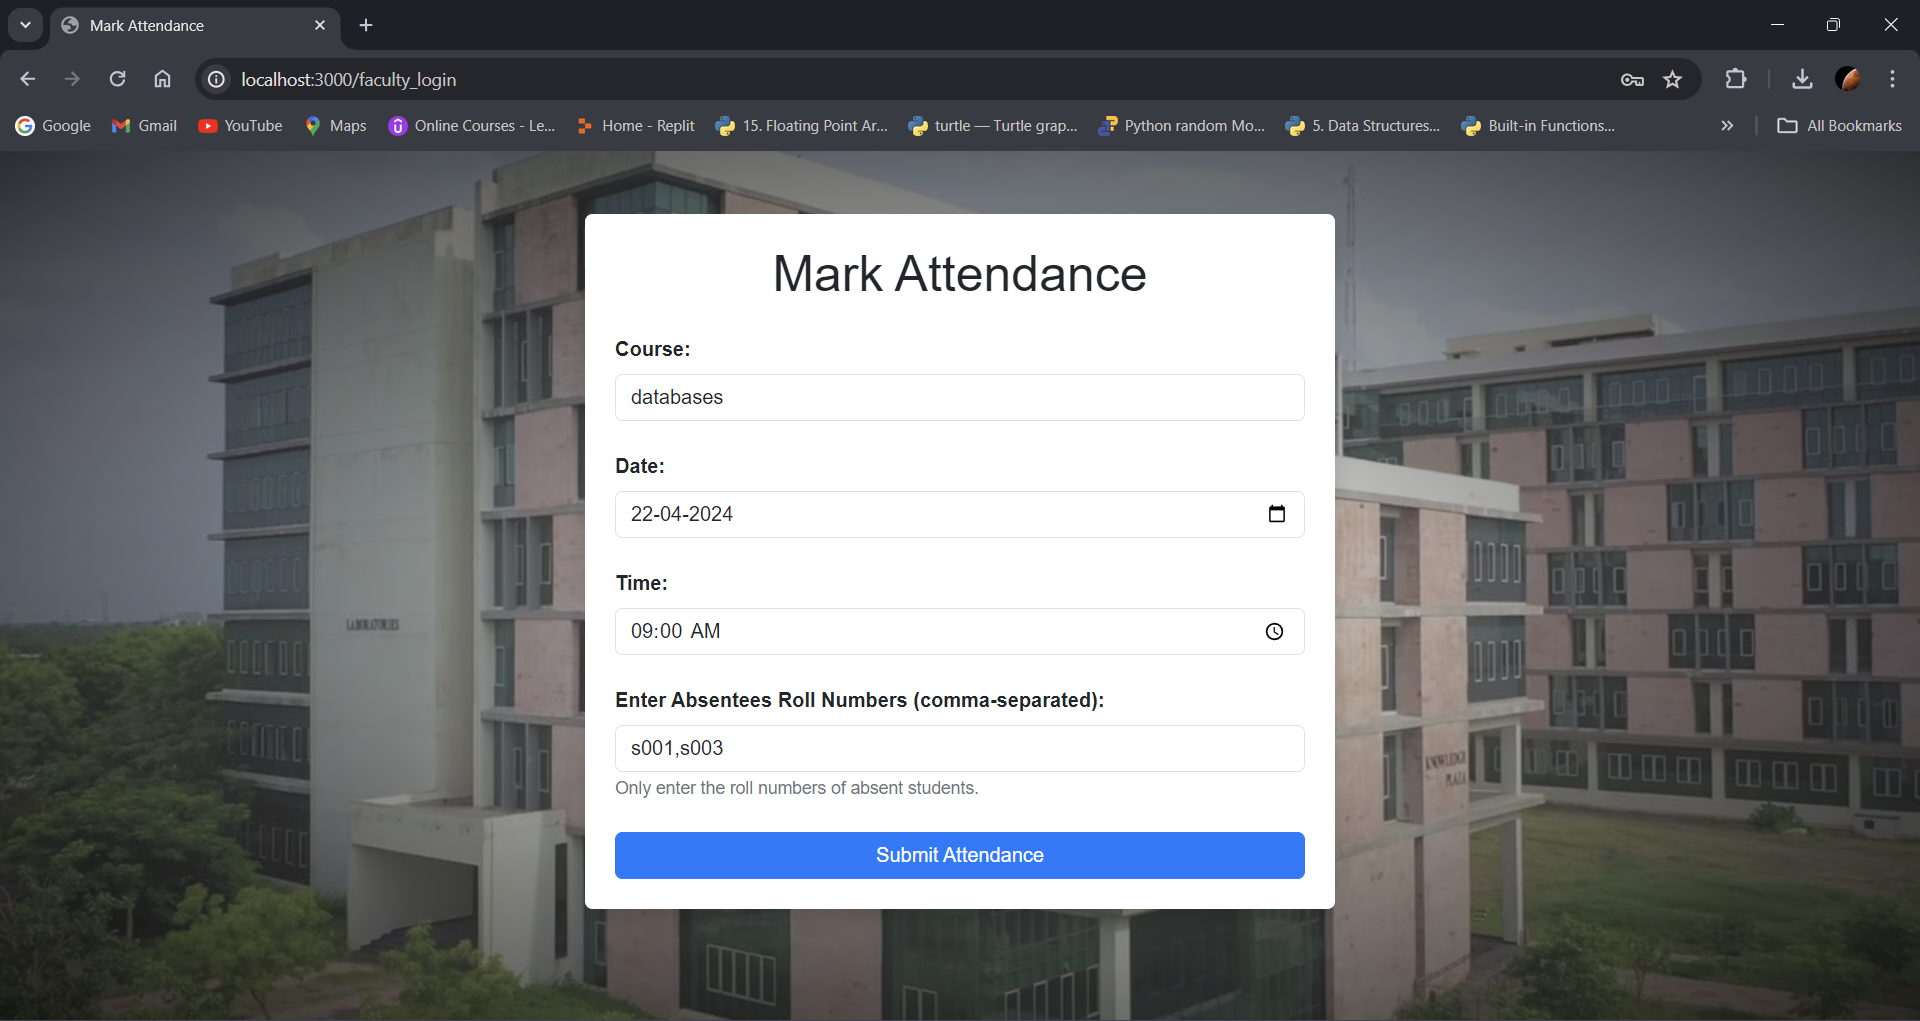
\includegraphics[width=1.1\textwidth, center]{18}
    \end{figure}

\end{itemize}


\newpage
\section*{\LARGE{Technology Stack used:}}
\begin{large}
\begin{enumerate}
    
    \item Front-End:
    \begin{itemize}
        \item HTML :  To design the structure of the webpages
        \item CSS : To style the webpages
        \item BootStrap : An external framework used for styling the webpages.
        \item Embedded JavaScript (EJS) : A templating language used to generate HTML markup with plain javascript.
    \end{itemize}
    
    \item Back-End:
    \begin{itemize}
        \item JavaScript : A scripting language used to 
            add functionalities to the webpages
        \item NodeJS : A javascript runtime environment used for executing javascript outside a web browser.
        \item ExpressJS :  Express is a node js web application framework that provides broad features for building web and mobile applications.
         It is used to build a single page, multipage, and hybrid web application. 
        \item MySQL : A Relational Database Management System. Used for storing various records. 
    \end{itemize}
\end{enumerate}
\end{large}


\section*{\LARGE{Methodology:}}
\begin{large}
    The front end has been created and designed using HTML and CSS. HTML has been used to give structure to the website.
    CSS and along with BootStrap, an external CSS framework are used for styling, positioning of elements of different webpages.

    \vspace*{0.5cm}

    \par
    Coming to the Back-end the website utilises javascript, NodeJS, ExpressJS for the creation of server which handle the requests coming
    from the webpages. Nodemon is an NodeJs framework which automatically restarts the .js file whenver there are any file changes occuring the
    directory.

    \vspace*{0.5cm}

    \par
    Using ExpressJS we create a server and host our website on the port 3000(say). So upon loading the website, we render the landing page of the application
    by sending a GET request to the server. Upon logging in by the student or faculty the website sends a POST request to the server.
    Then the server sends the appropriate webpage as a response for student and faculty. The website sends appropriate GET or POST requests based on the necessity 
    of the user. If something is to be shows or updated in the webpage, sending data securing in the request body (in case if forms) we use POST.
    GET is for fetching data.
    
    \vspace*{0.5cm}

    \par

    Using MySQL Querying we obtain the details of the student attendance by joining the required tables from the database.
    To Obtain the present classes of the student we use the following query:
    \newpage
    \begin{verbatim}
    SELECT 
        course.coursename, 
        CONCAT(instructor.instructorfname, ' ', instructor.instructormname,
            ' ', instructor.instructorlname) AS faculty_name,
        COUNT(class.classid) AS total_classes,
        SUM(CASE WHEN attends.attendancestatus = 'present' 
            THEN 1 ELSE 0 END) AS present_classes
    FROM 
        enrolls
        JOIN course ON enrolls.courseid = course.courseid
        JOIN instructs ON course.courseid = instructs.courseid
        JOIN instructor ON instructs.instructorid = instructor.instructorid
        JOIN class ON course.courseid = class.courseid AND 
            class.instructorid = instructor.instructorid
        LEFT JOIN attends ON class.classid = attends.classid AND 
            attends.studentid = ?
    WHERE 
        enrolls.studentid = ?
    GROUP BY 
        course.coursename, faculty_name 

    \end{verbatim}

    \vspace*{0.5cm}
    \par
    To get courses taught by a paricular instructor
    \begin{verbatim}
    SELECT course.courseid, course.coursename 
    FROM instructs 
    JOIN course ON instructs.courseid = course.courseid 
    WHERE instructs.instructorid = ?
    \end{verbatim}


    \vspace*{0.5cm}
    \par
    To get student details enrolled in a particular course:
    \begin{verbatim}
    SELECT student.studentid, student.fname, student.lname 
    FROM enrolls 
    JOIN student ON enrolls.studentid = student.studentid 
    WHERE enrolls.courseid = ?
    \end{verbatim}

    \vspace*{0.5cm}
    \par

    To mark attendance of the students wwe only enter the absentees roll number/student id 
    Attendance is marked as present for all other students. This is done by first initialising 
    attendance to "present" for all students and changing to "absent" for only those who are absent

    \newpage

    This is done by the following code:

    \begin{verbatim}
    absenteesArray= absentees?absentees.split(',').map(id => id.trim()):[];
    status= absenteesArray.includes(student.studentid)?'absent':'present';
    insertAttendanceQuery = `
        INSERT INTO attends (studentid,classid,attendancestatus,attendancedate)
        VALUES (?, ?, ?, ?)
        ON DUPLICATE KEY UPDATE attendancestatus=VALUES(attendancestatus)
        `;
    \end{verbatim}

    \vspace*{0.5cm}
    To get the leave requests of a particular student:
    \begin{verbatim}
    SELECT DATE_FORMAT(leavestartdate, '%Y-%m-%d') AS leavestartdate,
           DATE_FORMAT(leaveenddate, '%Y-%m-%d') AS leaveenddate,
           leavetype, leavereason, leavestatus
    FROM leaverequest
    WHERE studentid = ?
    \end{verbatim}  


\vspace*{1cm}
\bfseries{Below is code for Back-End: (app.js file)}
\begin{verbatim}
const express = require('express');
const mysql = require('mysql');
const app = express();
const session = require('express-session');
const cors = require('cors');
const port = 3000;

app.set('view engine', 'ejs');
app.use(express.static('public'));
app.use(express.urlencoded({ extended: true }));
app.use(cors());

app.use(session({
    secret: 'your secret key',
    resave: false,
    saveUninitialized: true
}));



const db = mysql.createConnection({
    host: 'localhost',
    user: 'root',
    password: 'Sumakar@mysql5',
    database: 'attendance'
});

db.connect(err => {
    if (err) {
        console.error('Database connection failed: ' + err.stack);
        return;
    }
        console.log('Connected to database.');
});

app.get('/', (req, res) => {
    res.render('landing');
});

app.get('/student_login', (req, res) => {
    res.render('student_login');
});

app.get('/faculty_login', (req, res) => {
    res.render('faculty_login');
});


app.post('/student_login', (req, res) => {
    const { username, password} = req.body;
    

    const query = 'SELECT * FROM user WHERE username = ? AND 
        passkey = ? AND usertype = "student"';
    db.query(query, [username, password], (err, results) => {
        if (err) throw err;

        

        if (results.length > 0) {
        const userId = results[0].userid;
        req.session.userid = userId;
        const studentQuery = 'SELECT * FROM student WHERE userid = ?';
        
        db.query(studentQuery, [userId], (err, studentResults) => {
            if (err) throw err;

            if (studentResults.length > 0) {
            const studentId = studentResults[0].studentid;
            const attendanceQuery = `
                SELECT 
                course.coursename, 
                CONCAT(instructor.instructorfname, ' ', 
                    instructor.instructormname, ' ',
                    instructor.instructorlname) AS faculty_name,
                COUNT(class.classid) AS total_classes,
                SUM(CASE WHEN attends.attendancestatus = 'present' 
                    THEN 1 ELSE 0 END) 
                    AS present_classes
                FROM 
                enrolls
                JOIN course ON enrolls.courseid = course.courseid
                JOIN instructs ON course.courseid = instructs.courseid
                JOIN instructor ON instructs.instructorid = 
                    instructor.instructorid
                JOIN class ON course.courseid = class.courseid AND 
                    class.instructorid = instructor.instructorid
                LEFT JOIN attends ON class.classid = attends.classid AND 
                    attends.studentid = ?
                WHERE 
                enrolls.studentid = ?
                GROUP BY 
                course.coursename, faculty_name
            `;

            db.query(attendanceQuery, [studentId, studentId], 
                (err, attendanceResults) => {
                    if (err) throw err;

                res.render('student_attendance', {student:studentResults[0], 
                    attendance:attendanceResults });
            });
            } else {
            res.send('Student not found.');
            }
        });
        } else {
        res.send('Invalid username or password');
        }
    });
});


app.post('/faculty_login', (req, res) => {
    const { username, password, userid } = req.body;

    const query = 'SELECT * FROM user WHERE username = ? AND 
        passkey = ? AND usertype = "teach"';
    db.query(query, [username, password], (err, results) => {
        if (err) throw err;

        if (results.length > 0) {
        const userId = results[0].userid;
        const facultyQuery = 'SELECT * FROM instructor WHERE userid = ?';
        
        db.query(facultyQuery, [userId], (err, facultyResults) => {
            if (err) throw err;

            if (facultyResults.length > 0) {
            const instructorId = facultyResults[0].instructorid;
            const coursesQuery = `
                SELECT course.courseid, course.coursename 
                FROM instructs 
                JOIN course ON instructs.courseid = course.courseid 
                WHERE instructs.instructorid = ?
            `;

            db.query(coursesQuery, [instructorId], (err, courses) => {
                if (err) throw err;

                res.render('mark_attendance', { instructorid: instructorId,
                    courses: courses });
            });
            } else {
            res.send('Faculty not found.');
            }
        });
        } else {
        res.send('Invalid username or password');
        }
    });
});



app.get('/get_students', (req, res) => {
    const { courseid } = req.query;

    const studentsQuery = `
        SELECT student.studentid, student.fname, student.lname 
        FROM enrolls 
        JOIN student ON enrolls.studentid = student.studentid 
        WHERE enrolls.courseid = ?
    `;

    db.query(studentsQuery, [courseid], (err, results) => {
        if (err) throw err;

        res.json(results);
    });
});



// Add this route to handle the form submission from mark_attendance.ejs
app.post('/mark_attendance', (req, res) => {
    const { instructorid, courseid, date, time, absentees } = req.body;

// Fetch all students enrolled in the selected course
    const enrolledStudentsQuery = `
        SELECT s.studentid
        FROM enrolls e
        JOIN student s ON e.studentid = s.studentid
        WHERE e.courseid = ?
    `;

    db.query(enrolledStudentsQuery, [courseid], (err, students) => {
        if (err) throw err;

        // Parse absentees from the request
        const absenteesArray=absentees?absentees.split(',').map(id=>id.trim()):[];

        // Fetch the class ID for the selected course, 
        // instructor, date, and time
        const classQuery = `
        SELECT classid FROM class 
        WHERE courseid = ? AND instructorid = ? AND 
            starttime <= ? AND endtime >= ?
        `;

        db.query(classQuery, [courseid, instructorid, 
            time, time], (err, classResults) => {
        if (err) throw err;

        if (classResults.length > 0) {
            const classid = classResults[0].classid;

            // Mark all students as present initially
            students.forEach(student => {
            const status = 
                absenteesArray.includes(student.studentid)?'absent':'present';
            const insertAttendanceQuery = `
                INSERT INTO 
                    attends (studentid,classid,attendancestatus,attendancedate)
                VALUES (?, ?, ?, ?)
                ON DUPLICATE KEY UPDATE 
                    attendancestatus = VALUES(attendancestatus)
            `;

            db.query(insertAttendanceQuery, 
                [student.studentid, classid, status, date], (err, results) => {
                if (err) throw err;
            });
            });

            res.send('Attendance marked successfully.');
        } else {
            res.send('Class not found.');
        }
        });
    });
});



app.get('/apply_leave', (req, res) => {
    const userid = req.session.userid;
    const query = `
    SELECT studentid
    FROM student
    WHERE userid = ?
    `;

    var studentID = ""
    db.query(query, [userid], (err, results) => {
        if (err) {
        console.error('Error retrieving student ID:', err);
        res.sendStatus(500); 
        return;
        }
    
        if (results.length === 0) {
        console.log('Student ID not found for user ID:', userid);
        res.sendStatus(404);
        return;
        }
    
        studentID = results[0].studentid;  
    });

    const studentQuery = `
        SELECT s.fname, s.lname, s.studentid, s.department
        FROM student s
        WHERE s.userid = ?
    `;
    db.query(studentQuery, [userid], (err, studentResult) => {
        if (err) {
            console.error('Error fetching student details:', err);
            res.sendStatus(500);
            return;
        }      
        
        if (!studentResult[0]) {
            res.render('apply_leave', { student: null });
        } else {
            res.render('apply_leave', { student: studentResult[0] });
        }
    });
 });




app.get('/apply_leave', (req, res) => {
    const userid = req.session.userid;
    
    var studentID = ""
    db.query(query, [userid], (err, results) => {
        if (err) {
        console.error('Error retrieving student ID:', err);
        res.sendStatus(500); 
        return;
        }
    
        if (results.length === 0) {
        console.log('Student ID not found for user ID:', userid);
        res.sendStatus(404);
        return;
        }
    
        studentID = results[0].studentid;  
        req.session.studentID = studentID
    });

    const studentQuery = `
        SELECT s.fname, s.lname, s.studentid, s.department
        FROM student s
        WHERE s.userid = ?
    `;
    db.query(studentQuery, [userid], (err, studentResult) => {
        if (err) {
        console.error('Error fetching student details:', err);
        res.sendStatus(500);
        return;
        }

        if (!studentResult || studentResult.length === 0) {
        console.error('No student details found.');
        res.render('apply_leave', { student: null });
        return;
        }

        res.render('apply_leave', { student: studentResult[0] });
    });
});





app.post('/apply_leave', (req, res) => {
    const userid = req.session.userid;
    const query = `
        SELECT studentid
        FROM student
        WHERE userid = ?
    `;
    db.query(query, [userid], (err, results) => {
        if (err) {
        console.error('Error retrieving student ID:', err);
        res.sendStatus(500);
        return;
        }
        if (results.length === 0) {
        console.log('Student ID not found for user ID:', userid);
        res.sendStatus(404);
        return;
        }
        const studentID = results[0].studentid;

        const { startDate, endDate, reason, type } = req.body;

        const latestLeaveRequestQuery = `
        SELECT leavereqid
        FROM leaverequest
        ORDER BY leavereqid DESC
        LIMIT 1
        `;
        db.query(latestLeaveRequestQuery, (err, results) => {
        if (err) {
            console.error('Error retrieving latest leave request ID:', err);
            res.sendStatus(500);
            return;
        }

        let latestRequestId = 0;
        if (results.length > 0) {
            latestRequestId = parseInt(results[0].leavereqid.substr(1));
        }

        const newRequestId = 'l' + ('000' + (latestRequestId + 1)).slice(-3);

        const stts = 'pending';

        const insertLeaveQuery = `
            INSERT INTO leaverequest (leavereqid, studentid, leavestartdate,
                leaveenddate, leavetype, leavereason, leavestatus)
            VALUES (?, ?, ?, ?, ?, ?, ?)
        `;

        db.query(insertLeaveQuery, [newRequestId, studentID, 
            startDate, endDate, type, reason, stts], (err, result) => {
            if (err) {
            console.error('Error inserting leave request:', err);
            res.sendStatus(500);
            return;
            }

            res.send('Leave request inserted successfully');
        });
        });
});
});



app.get('/leave_history', (req, res) => {
    const userid = req.session.userid;

    const query1 = `
        SELECT studentid
        FROM student
        WHERE userid = ?
    `;

    db.query(query1, [userid], (err, results) => {
        if (err) {
        console.error('Error retrieving student ID:', err);
        res.sendStatus(500);
        return;
        }

        if (results.length === 0) {
        console.log('Student ID not found for user ID:', userid);
        res.sendStatus(404);
        return;
        }

        const studentID = results[0].studentid;  

        const query = `
        SELECT DATE_FORMAT(leavestartdate, '%Y-%m-%d') AS leavestartdate,
                DATE_FORMAT(leaveenddate, '%Y-%m-%d') AS leaveenddate,
                leavetype, leavereason, leavestatus
        FROM leaverequest
        WHERE studentid = ?
        `;

        db.query(query, [studentID], (err, results) => {
        if (err) {
            console.error('Error retrieving leave history:', err);
            res.sendStatus(500); 
            return;
        }
        res.render('leave_history', { leaves: results });
        });
    });
});


app.listen(port, () => {
    console.log(`Server running at http://localhost:${port}`);
});

\end{verbatim}
\end{large}
\end{document}
